\subsection{Example: Extractions}
\label{sec:extraction}

The goal of this section is to provide a step-by-step description of the parasitic extraction process for future reference. Other students may find a tutorial of this kind helpful just as it is a good baseline for our upcoming work. \\

It was possible to extract parasitic inductance and resistance between various points within the nets. The following presents the step-by-step method of extracting the parasitic between two points, Q1 Drain and C11, that lies in one net, the DC+. Using a similar method, parasitic throughout different branches of the circuit were later extracted. The values are then added to the SPICE model for analyses.\\

\subsubsection{Setting up}

\begin{enumerate}
\item A schematic of one leg of a DC-DC converter was provided. It was studied to understand the scope of analysis. For the project, it was used as an inverter for the reasons laid out in Section \ref{sec:overview}.


\begin{figure} [H]
  \centering
  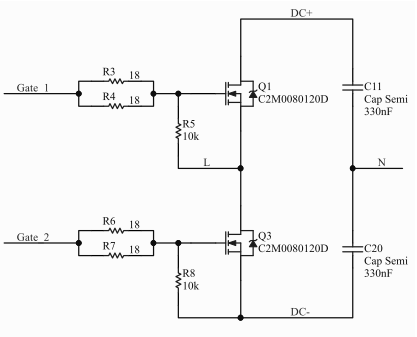
\includegraphics[width=\linewidth]{pictures/examples/main_schematic}
  \caption{Main Schematic of the circuit}
  \label{fig:main_schematic}
\end{figure}

\item A spice model was created based on the schematic which will be used to analyze the circuit once parasitic components from various branches of the circuit are extracted.

\begin{figure} [H]
  \centering
  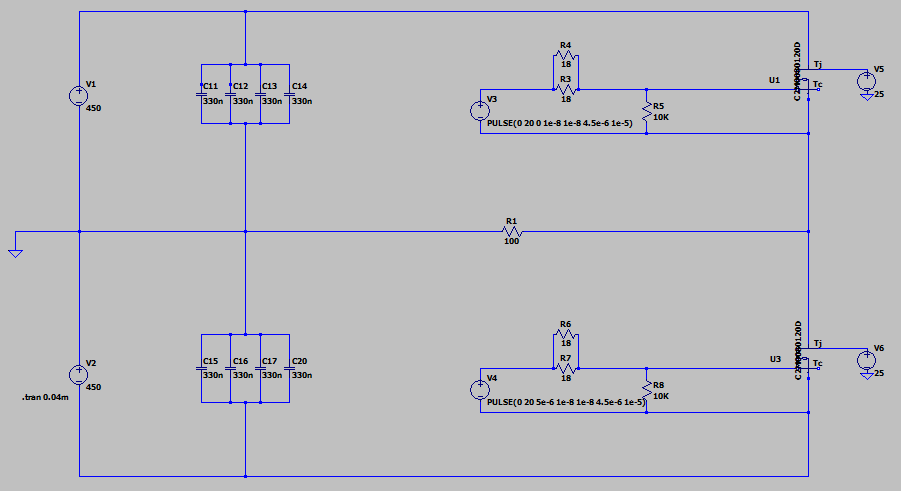
\includegraphics[width=\linewidth]{pictures/examples/spice.png}
  \caption{SPICE Model}
  \label{fig:main_spice}
\end{figure}

\item A 3D PCB Graphics layout was provided in PDF to identify the various components of the model. Analysis is not possible on this layout. It is provided only for component identification.

\begin{figure} [H]
  \centering
  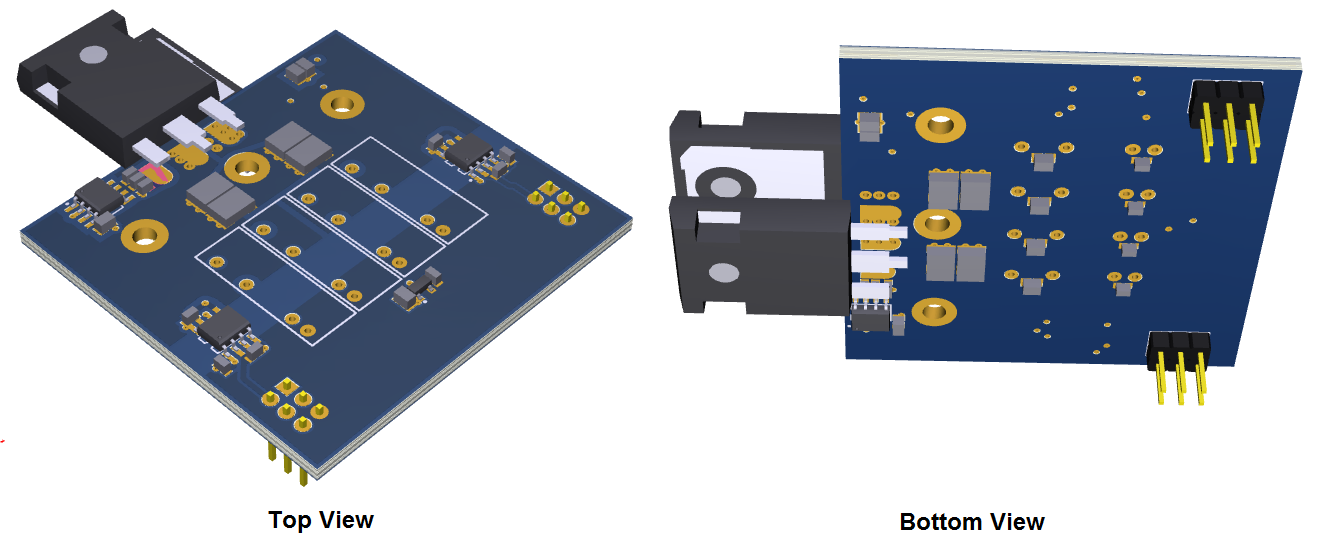
\includegraphics[width=\linewidth]{pictures/examples/PCB.png}
  \caption{3D PCB Layout in PDF}
  \label{fig:pcb}
\end{figure}

\item ODB++ files were provided which were imported to ANSYS SIwave to create the working 3D PCB Layout. Actual analysis is done on this layout.

\begin{figure} [H]
  \centering
  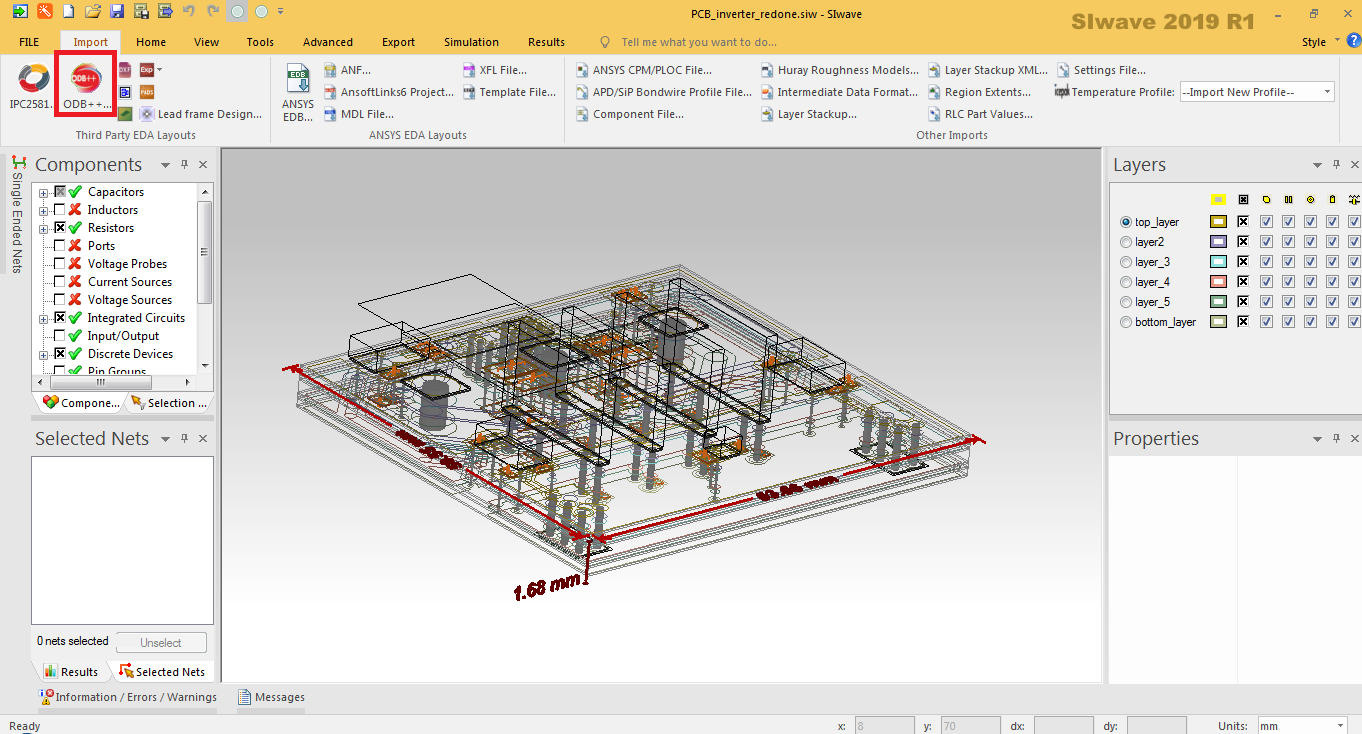
\includegraphics[width=\linewidth]{pictures/examples/siwave.png}
  \caption{ODB++ imported to create 3D PCB layout in ANSYS SIwave}
  \label{fig:siwave}
\end{figure}

\item The part of interest was cut from the 3D PCB layout and exported to Q3D extractor for extracting the values of the parasitic components.

\begin{figure} [H]
  \centering
  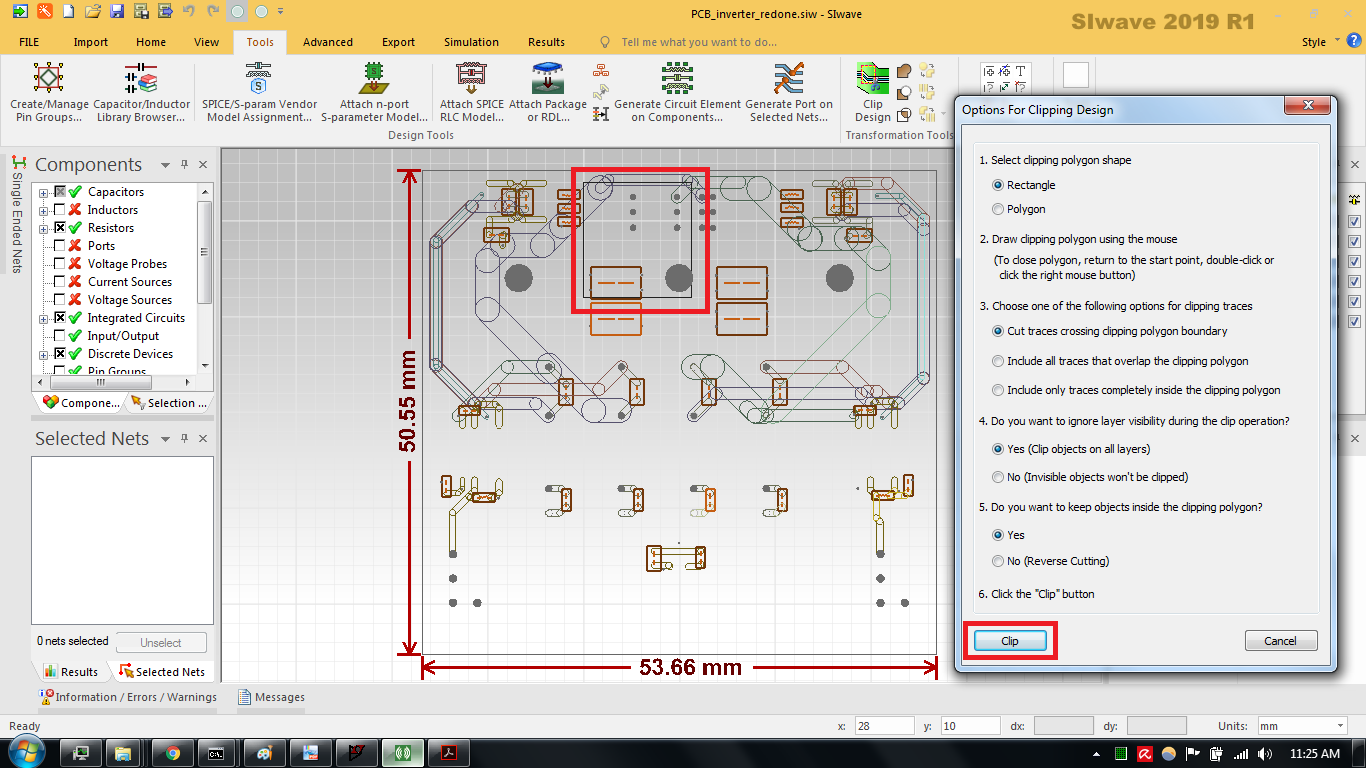
\includegraphics[width=\linewidth]{pictures/examples/siwave_clip2.png}
  \caption{The red box indicates the part of interest which will be cut and extracted to Q3D Extractor}
  \label{fig:siwave_cut}
\end{figure}

\end{enumerate}

\subsubsection{Step-by-step extraction process for parasitic inductance and resistance between Q1-Drain and C11 in the DC+ Net}

\begin{enumerate}
\item  First, we need to identify the two point in the schematic between which the parasitic is to be extracted. The points of interest must be in the same net. It is seen that the part of interest is the branch from Q1-Drain to C11 connected by the DC+ net.

\begin{figure} [H]
  \centering
  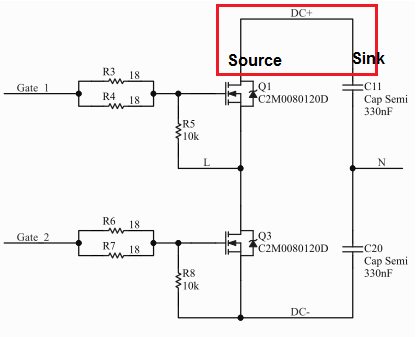
\includegraphics[width=\linewidth]{pictures/examples/Schematic1.png}
  \caption{The red box indicates the portion from where parasitic is extracted}
  \label{fig:schematic1}
\end{figure}

\item  The target is also marked in the corresponding SPICE model since the extracted parasitic components will be included in this particular branch.

\begin{figure} [H]
  \centering
  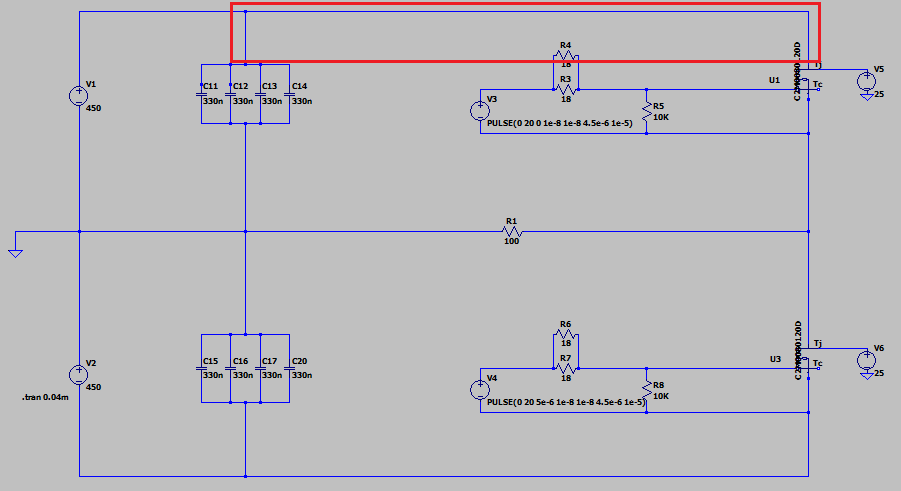
\includegraphics[width=\linewidth]{pictures/examples/spice1.png}
  \caption{The red box indicates the portion where the extracted parasitic is to be placed}
  \label{fig:spice1}
\end{figure}

\item Figure \ref{fig:PCB_cut1} depicts the section of the PDF PCB layout to be used for extraction. It shows the areas of Q1 drain and C11 on net DC+, while all other components are ignored. 

\begin{figure} [H]
  \centering
  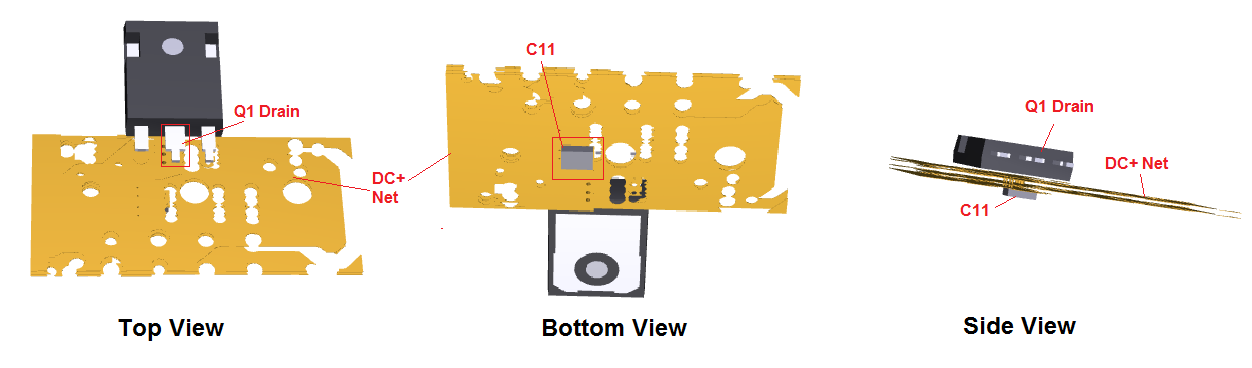
\includegraphics[width=\linewidth]{pictures/examples/PCB_cut_1.png}
  \caption{Portion of PCB that is of concern}
  \label{fig:PCB_cut1}
\end{figure}

\item Next, the PDF graphics layout is used to identify the part of interest within the net DC+ where the areas Q1-Drain and C11 are located in the ANSYS SIwave 3D PCB layout and that portion is clipped.

\begin{figure} [H]
  \centering
  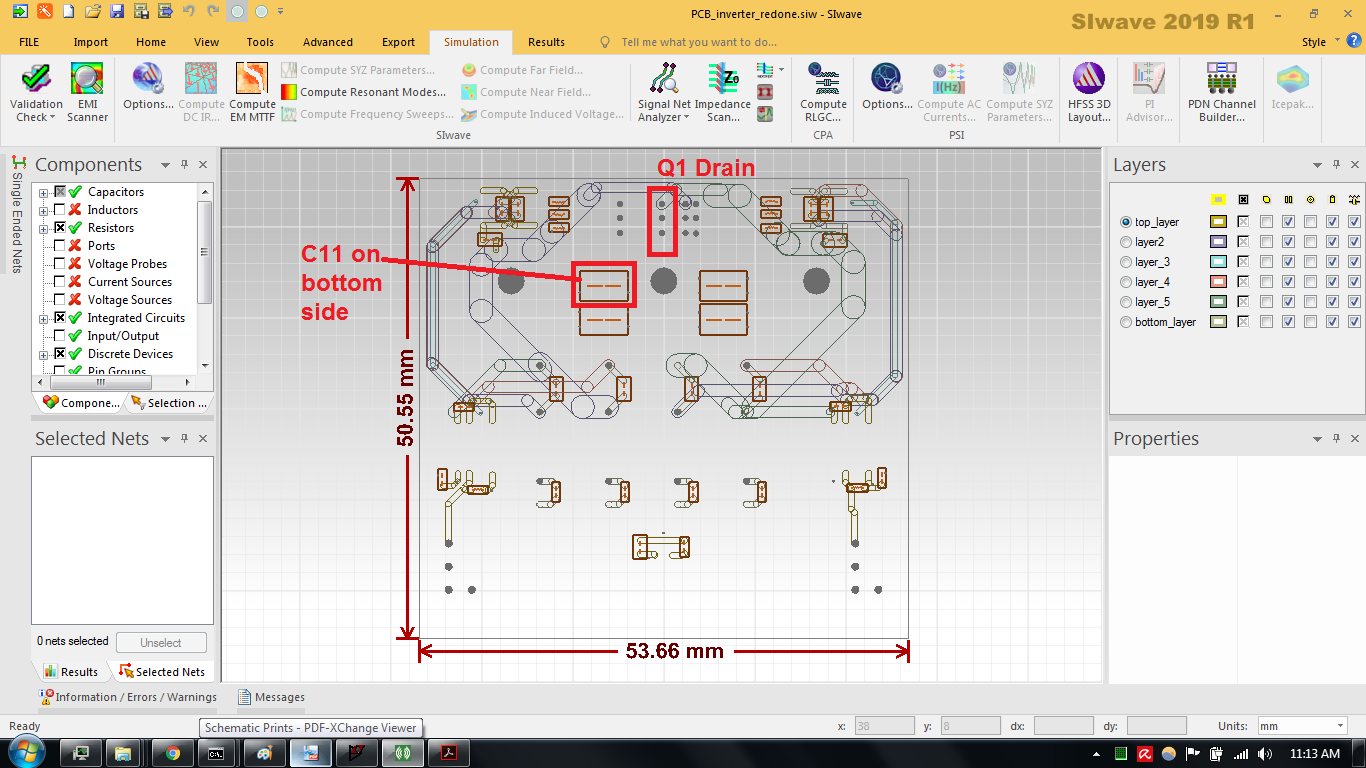
\includegraphics[width=\linewidth]{pictures/examples/siwave_td.png}
  \caption{Identifying Q1-Drain and C11 from top-down view}
  \label{fig:PCB_identify1}
\end{figure}

\begin{figure} [H]
  \centering
  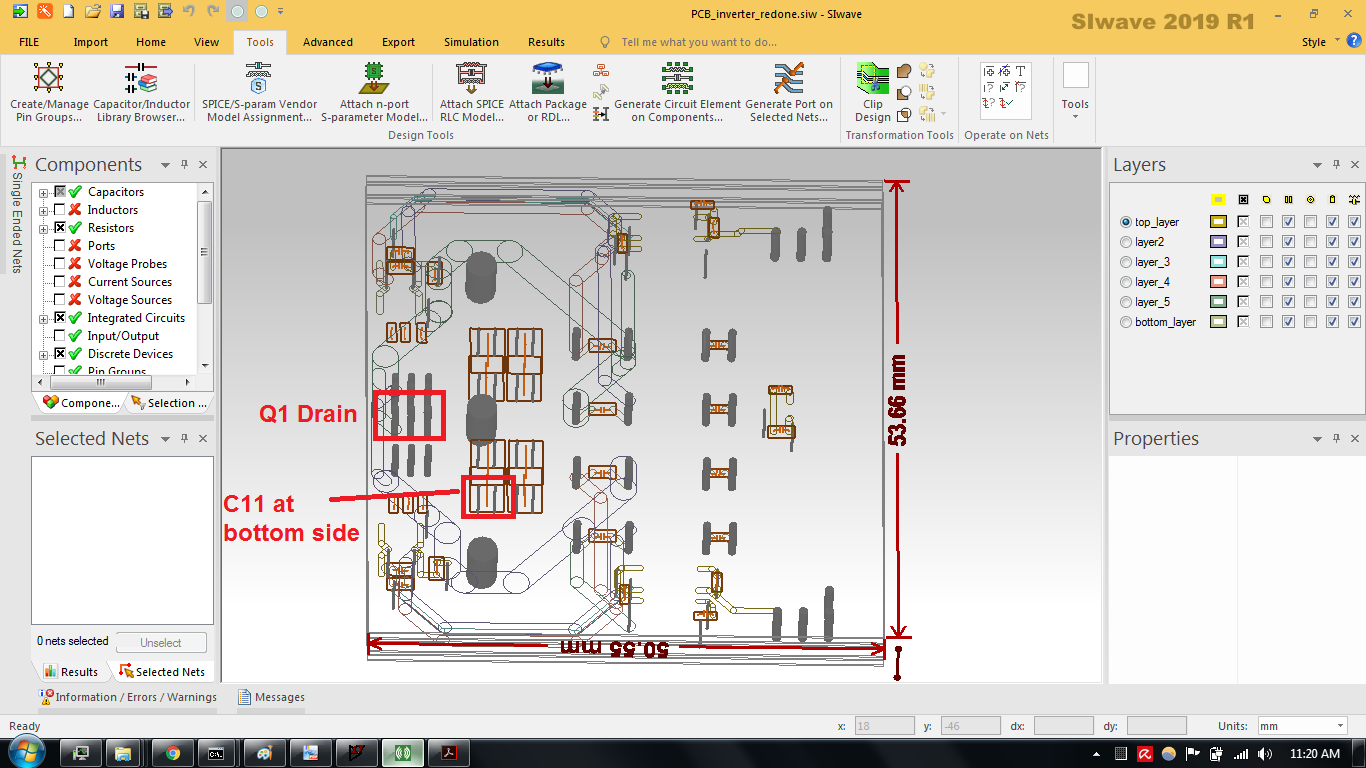
\includegraphics[width=\linewidth]{pictures/examples/siwave_ls.png}
  \caption{Identifying Q1-Drain and C11 from left side view}
  \label{fig:PCB_clip1}
\end{figure}

\begin{figure} [H]
  \centering
  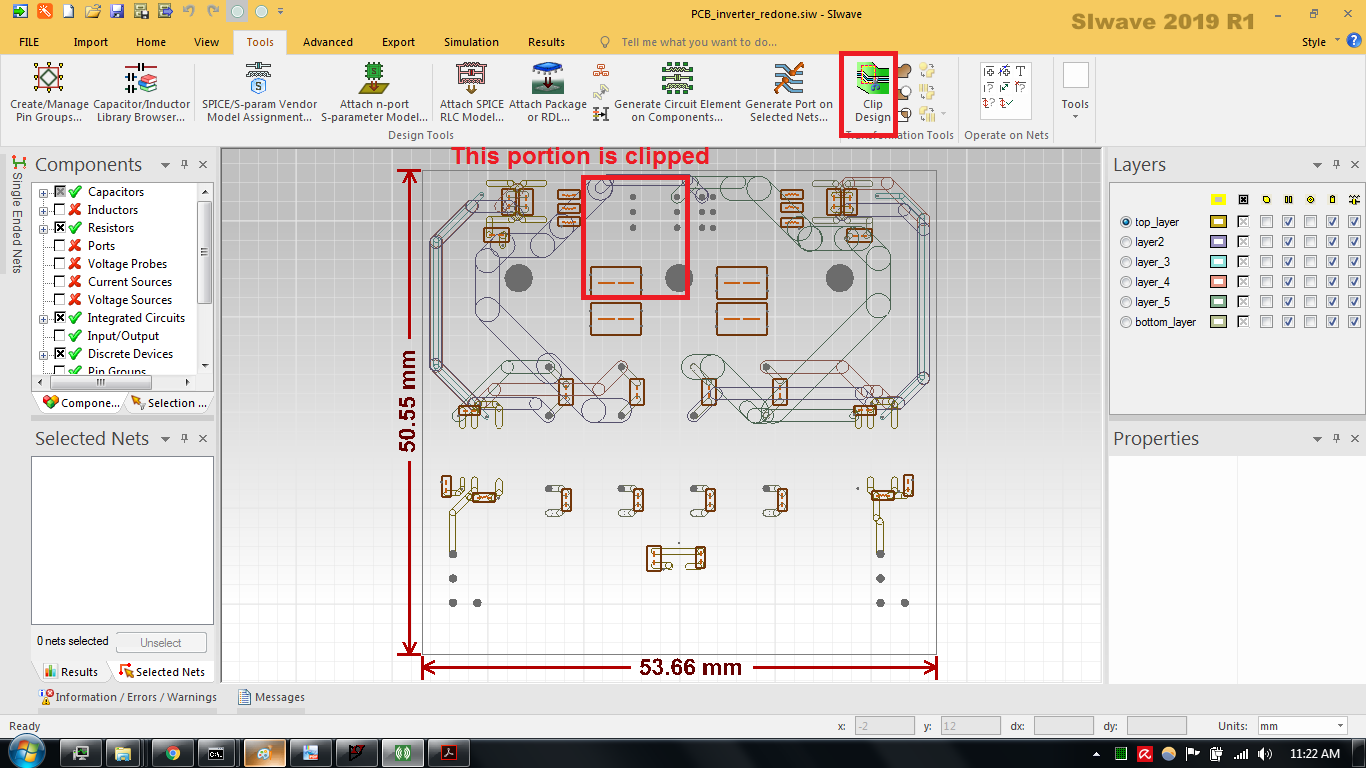
\includegraphics[width=\linewidth]{pictures/examples/siwave_clip1.png}
  \caption{Portion of PCB that is of concern containing all identified parts}
  \label{fig:PCB_clip1}
\end{figure}

\begin{figure} [H]
  \centering
  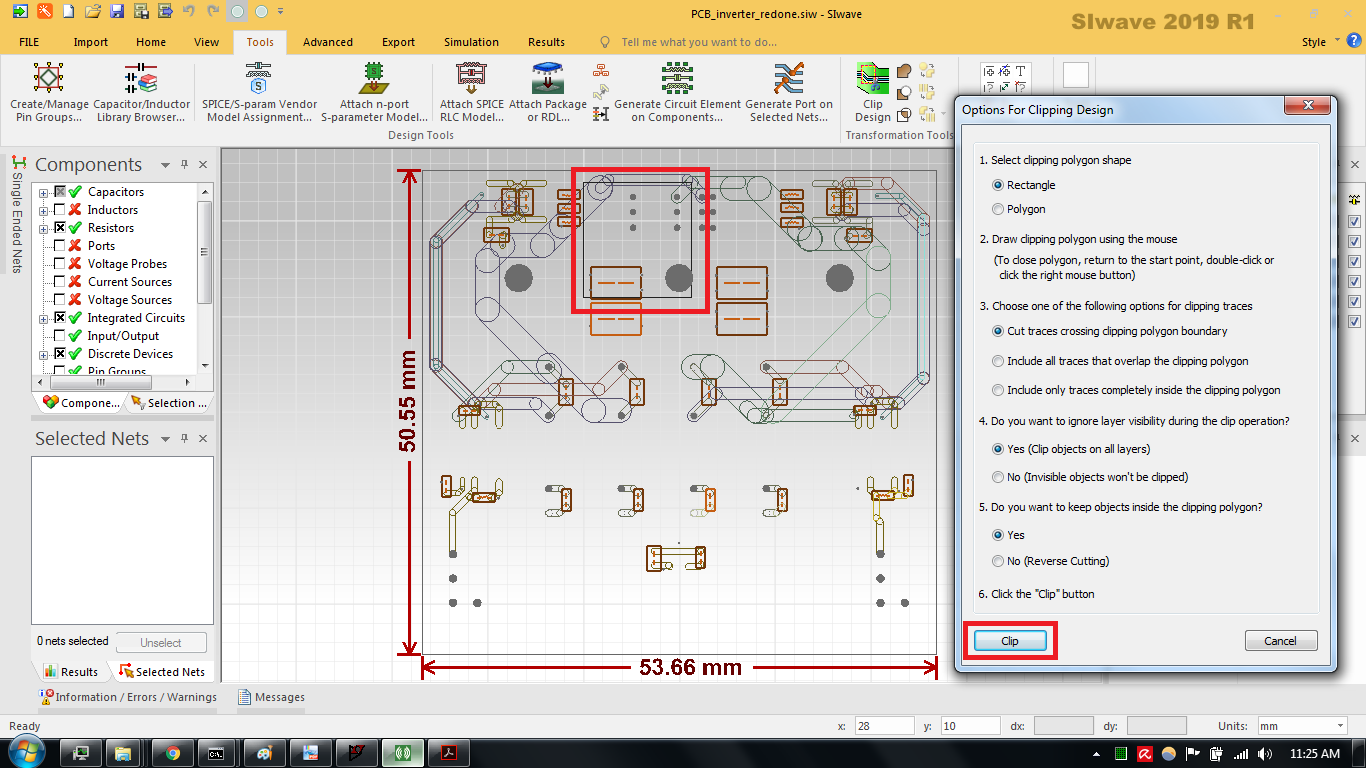
\includegraphics[width=\linewidth]{pictures/examples/siwave_clip2.png}
  \caption{Identified portion of PCB is clipped}
  \label{fig:PCB_clip2}
\end{figure}

\begin{figure} [H]
  \centering
  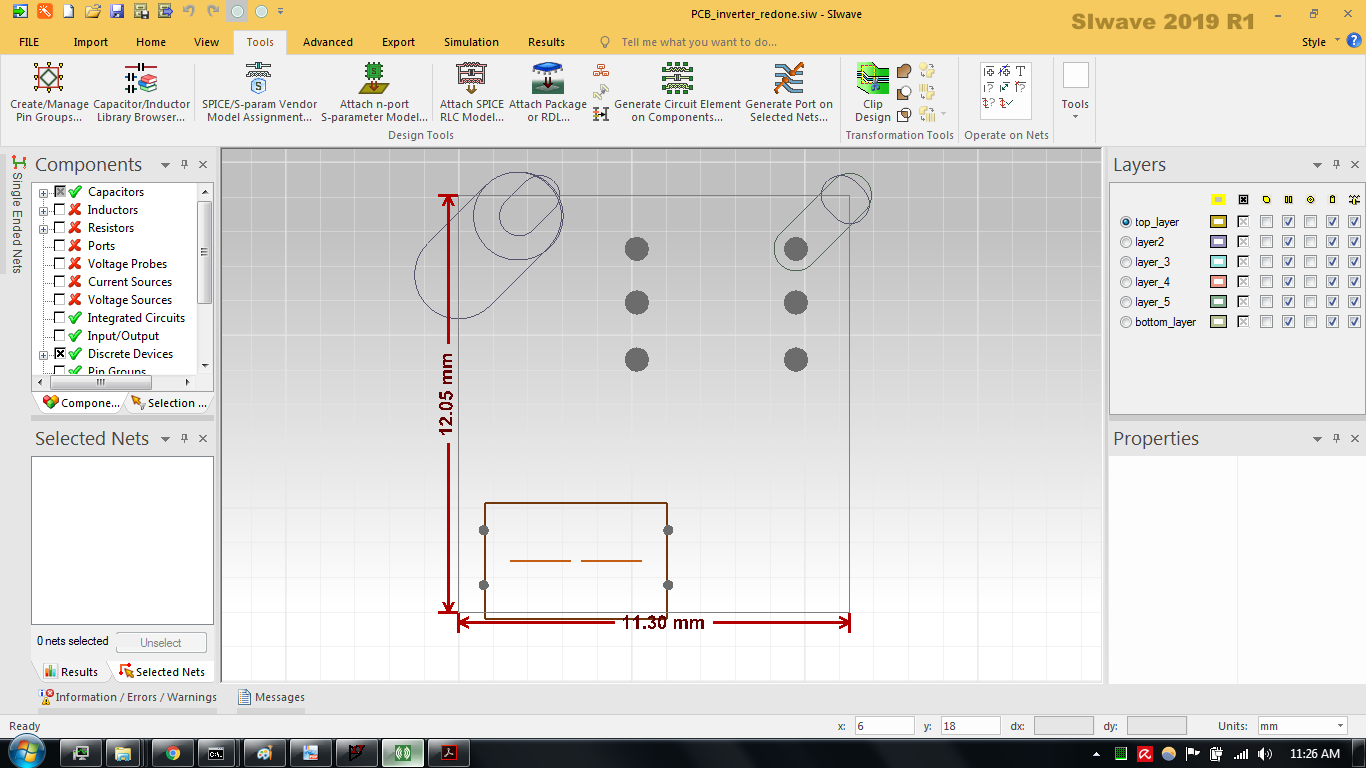
\includegraphics[width=\linewidth]{pictures/examples/siwave_clipped_td.png}
  \caption{Clipped part of the original PCB layout}
  \label{fig:PCB_clipped}
\end{figure}

\item The clipped portion is properly checked and verified to contain the part of interest. Repeat step 4 if clipping seems to have an error.

\begin{figure} [H]
  \centering
  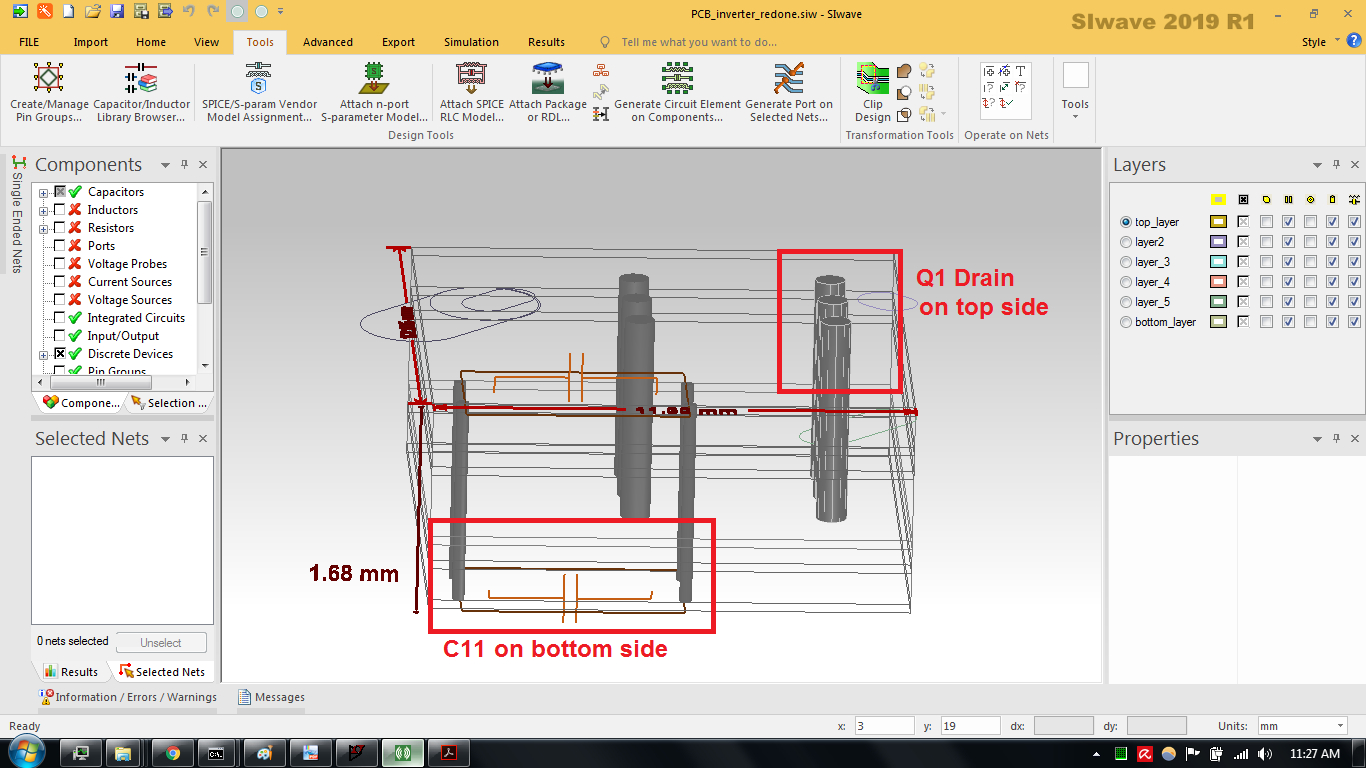
\includegraphics[width=\linewidth]{pictures/examples/siwave_clipped_side.png}
  \caption{Verifying the clipped part of the original PCB layout}
  \label{fig:PCB_verified}
\end{figure}

\item The clipped portion is exported to ANSYS Q3D Extractor to extract the parasitic components.

\begin{figure} [H]
  \centering
  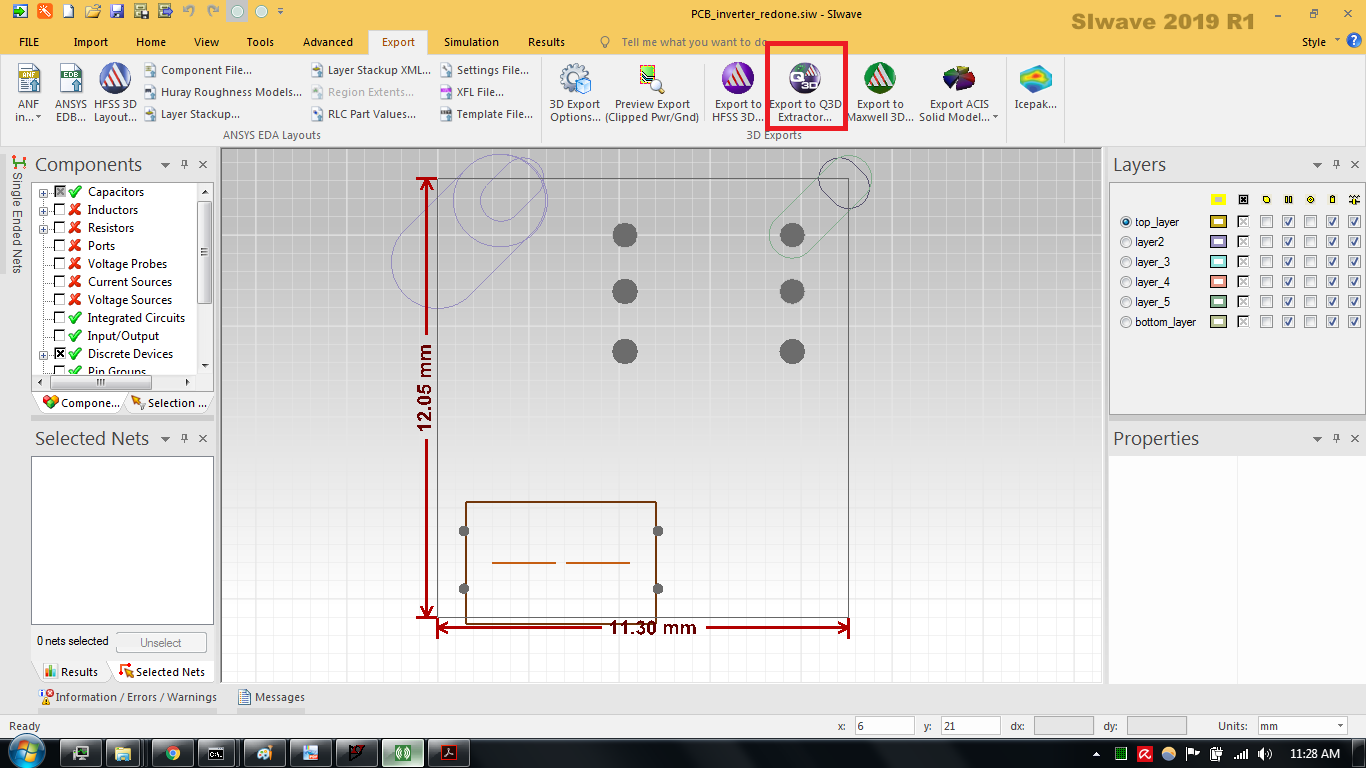
\includegraphics[width=\linewidth]{pictures/examples/siwave_export_q3d.png}
  \caption{Clipped PCB part is exported to ANSYS Q3D}
  \label{fig:siwave_q3d}
\end{figure}

\begin{figure} [H]
  \centering
  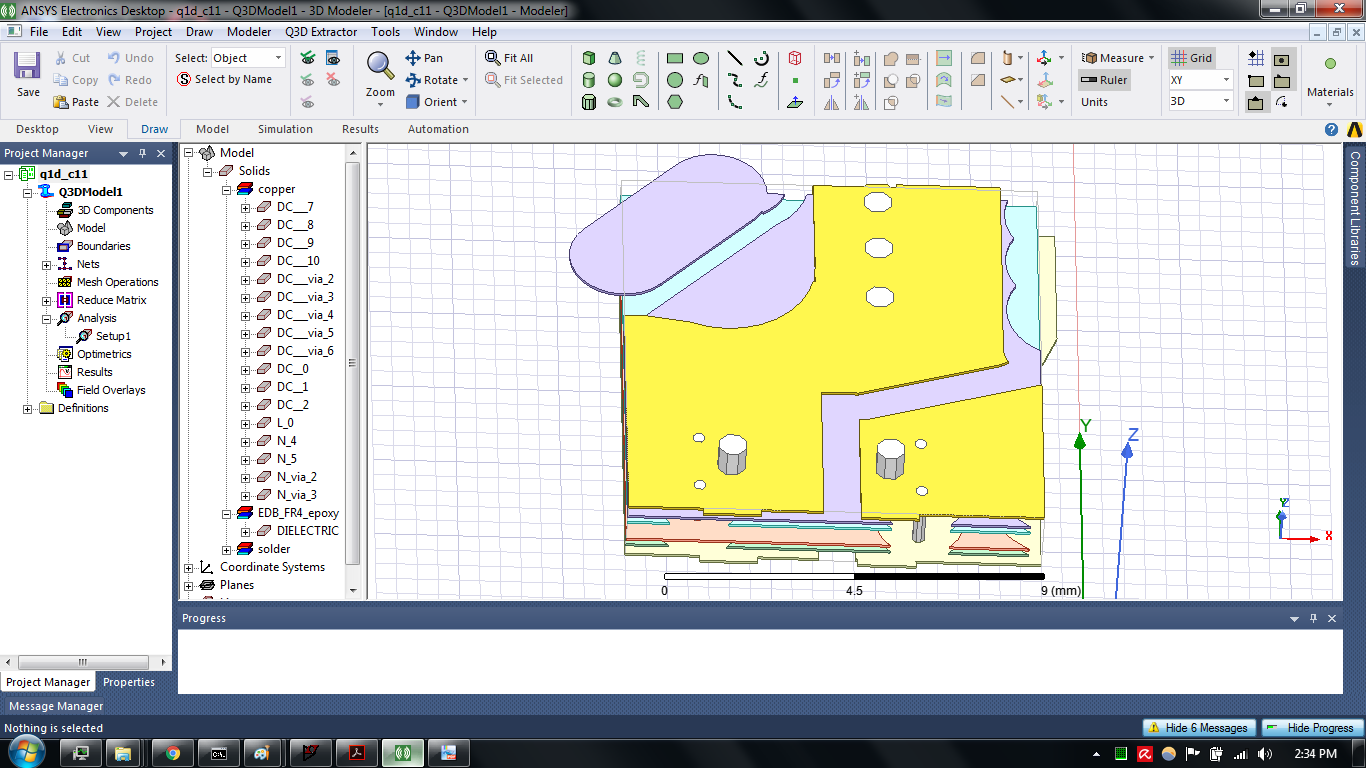
\includegraphics[width=\linewidth]{pictures/examples/Q1d_C11T_1.png}
  \caption{Top View of PCB Layout in Q3D}
  \label{fig:q3d1}
\end{figure}

\begin{figure} [H]
  \centering
  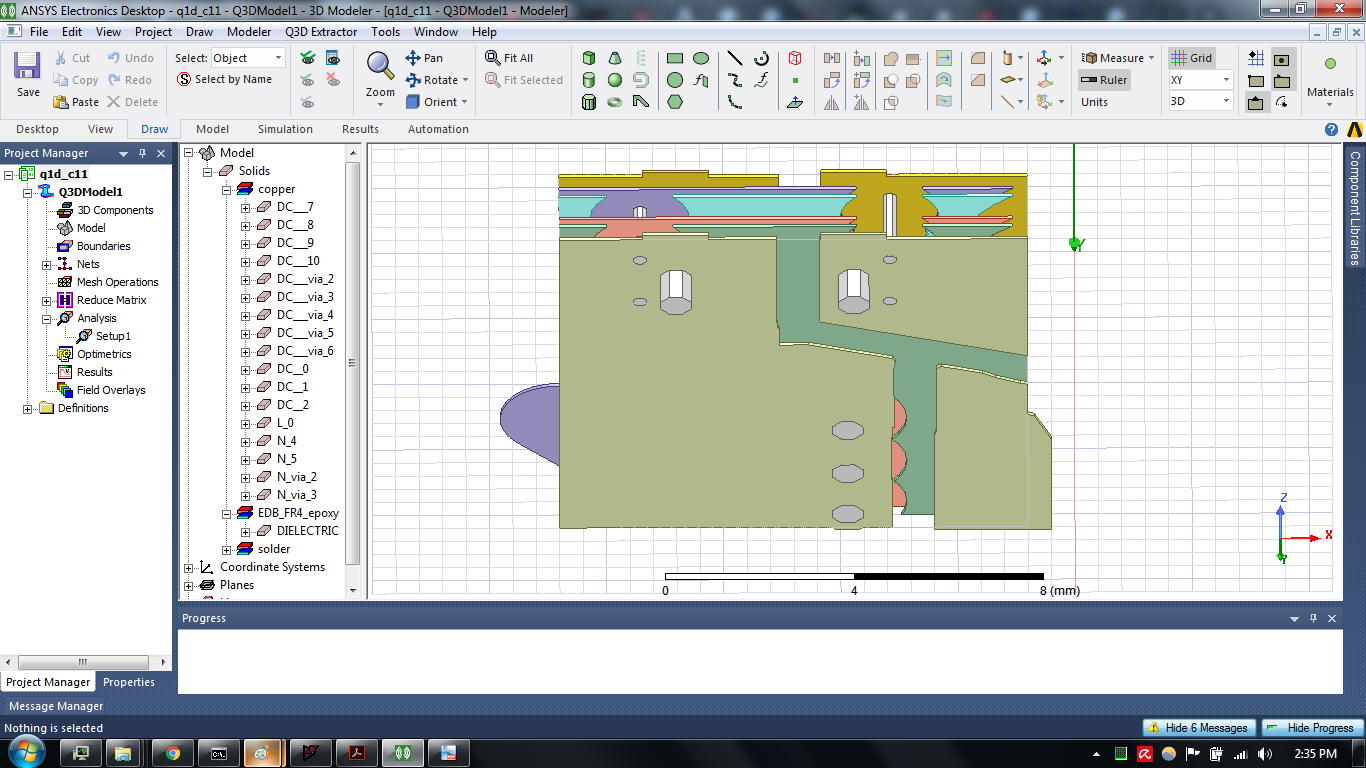
\includegraphics[width=\linewidth]{pictures/examples/Q1d_C11T_2.png}
  \caption{Bottom View of PCB Layout in Q3D}
  \label{fig:q3d2}
\end{figure}

\item In ANSYS Q3D, clipped PCB part containing the net DC+ is analyzed to recover the parasitic components\\

To find the parasitic components, we need to cover:
\begin{enumerate}
\item The area of the Q1-Drain and 
\item The area of the C11
\end{enumerate}
with a sheet on top of their individual located surfaces. The sheet has to be made of the same material as the face on which it is being created. In this case, it was copper.

\begin{figure} [H]
  \centering
  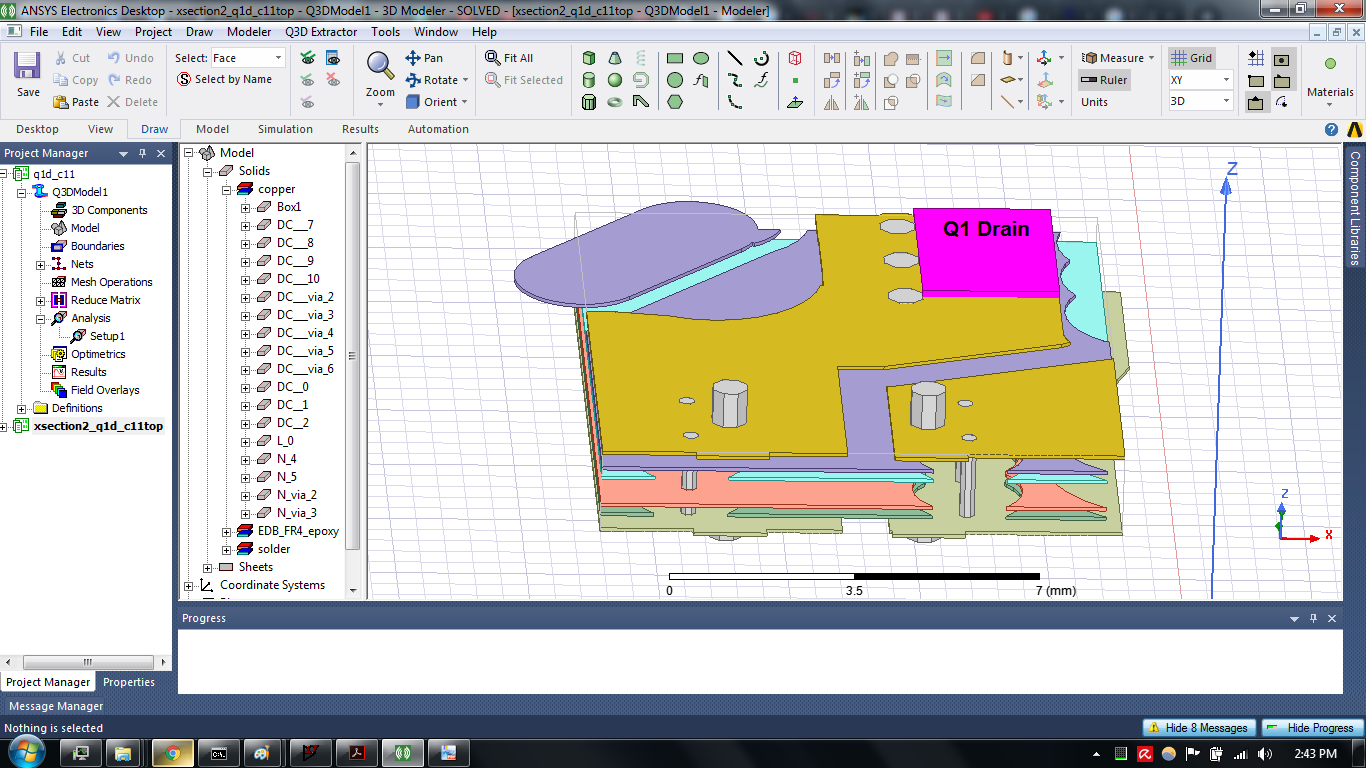
\includegraphics[width=\linewidth]{pictures/examples/Q1d_C11T_5.png}
  \caption{Q1-Drain area in the DC+ Net}
  \label{fig:Q1d}
\end{figure}

\begin{figure} [H]
  \centering
  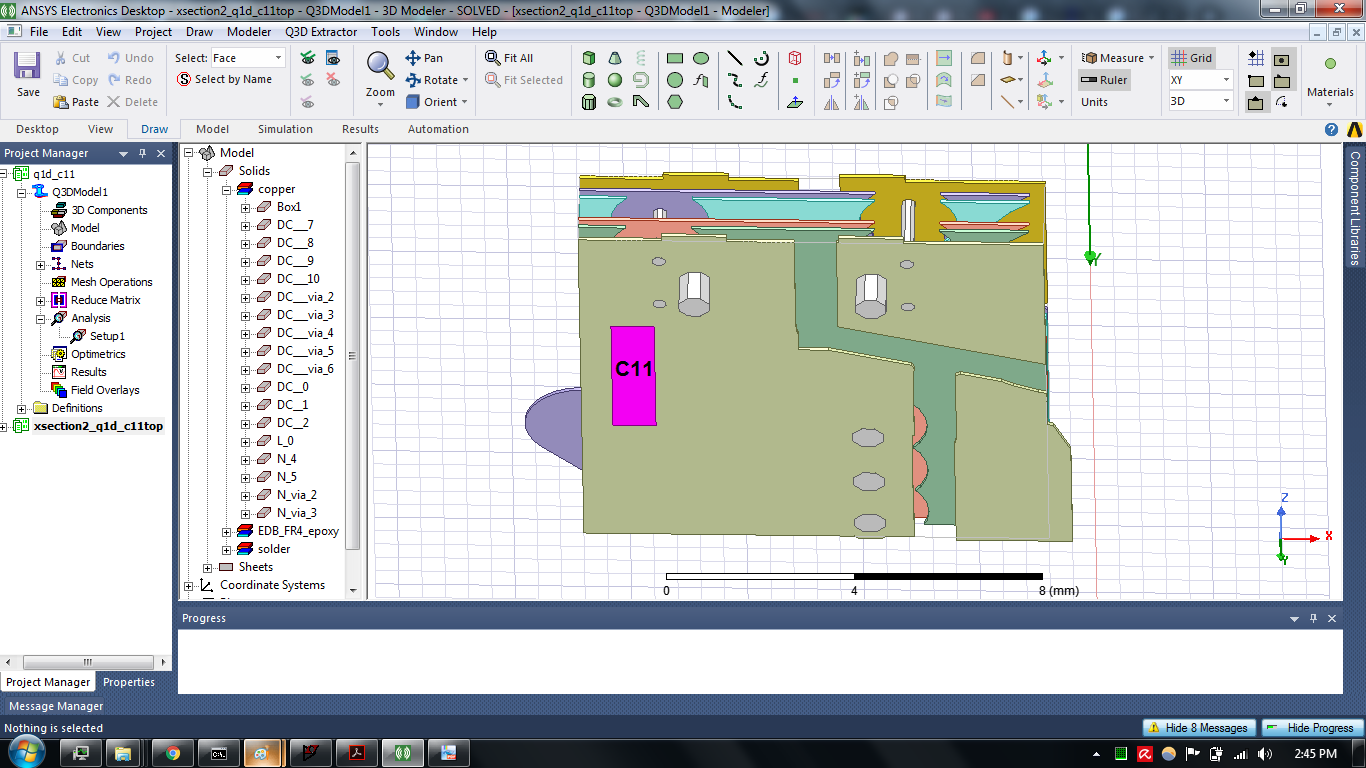
\includegraphics[width=\linewidth]{pictures/examples/Q1d_C11T_6.png}
  \caption{C11 area in the DC+ Net}
  \label{fig:Q1d_C11t_sink}
\end{figure}

\item Assigning excitation, one of the two sheets is marked as source and the other as sink.

\begin{figure} [H]
  \centering
  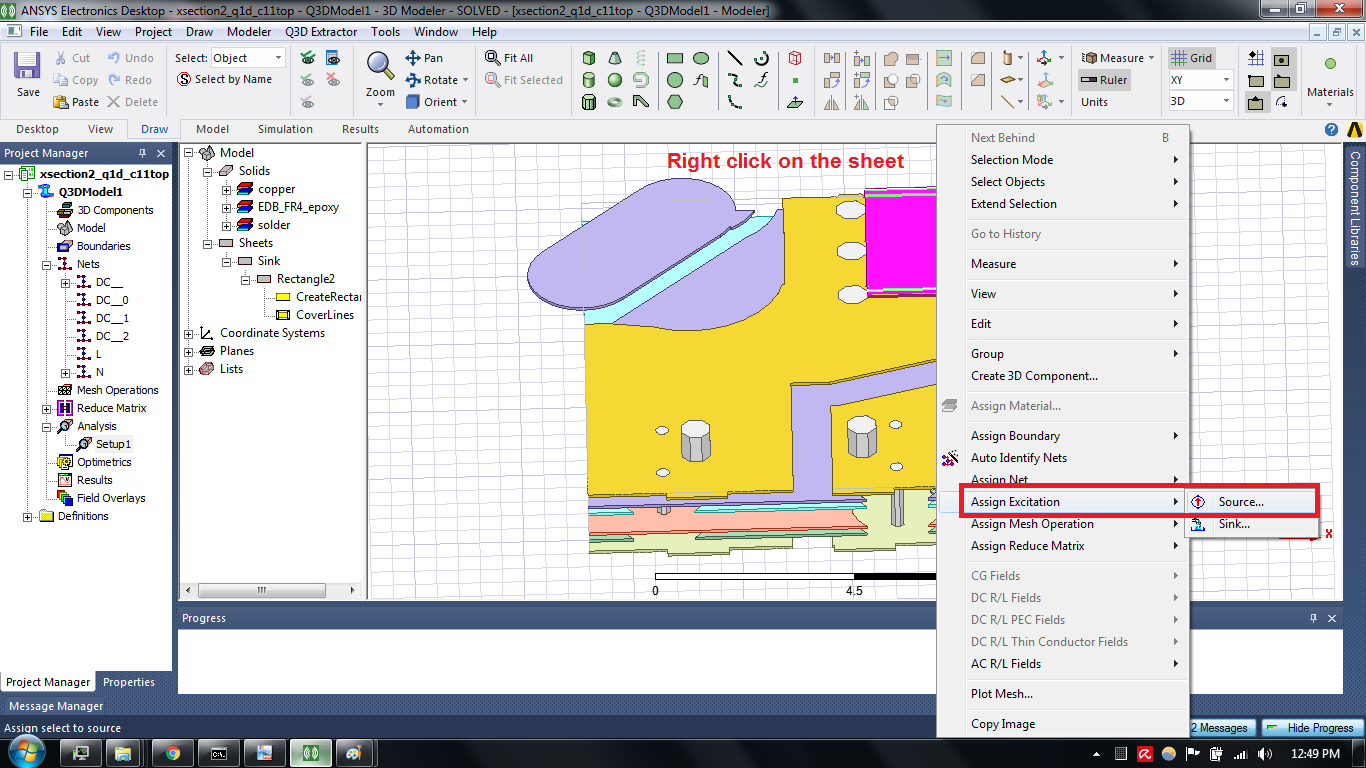
\includegraphics[width=\linewidth]{pictures/examples/source.png}
  \caption{Assigning Source to Q1-Drain}
  \label{fig:source1}
\end{figure}

\begin{figure} [H]
  \centering
  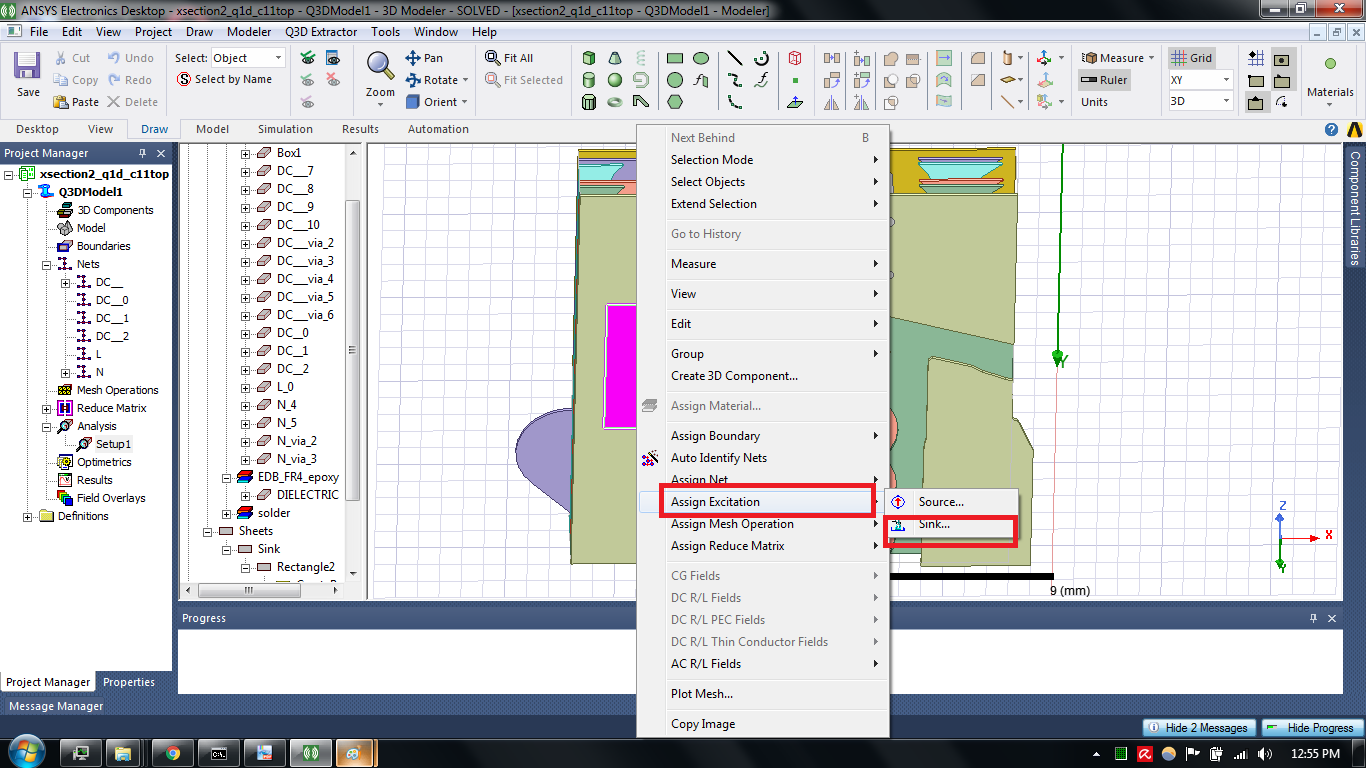
\includegraphics[width=\linewidth]{pictures/examples/sink.png}
  \caption{Assigning Sink to C11}
  \label{fig:sink1}
\end{figure}

\begin{figure} [H]
  \centering
  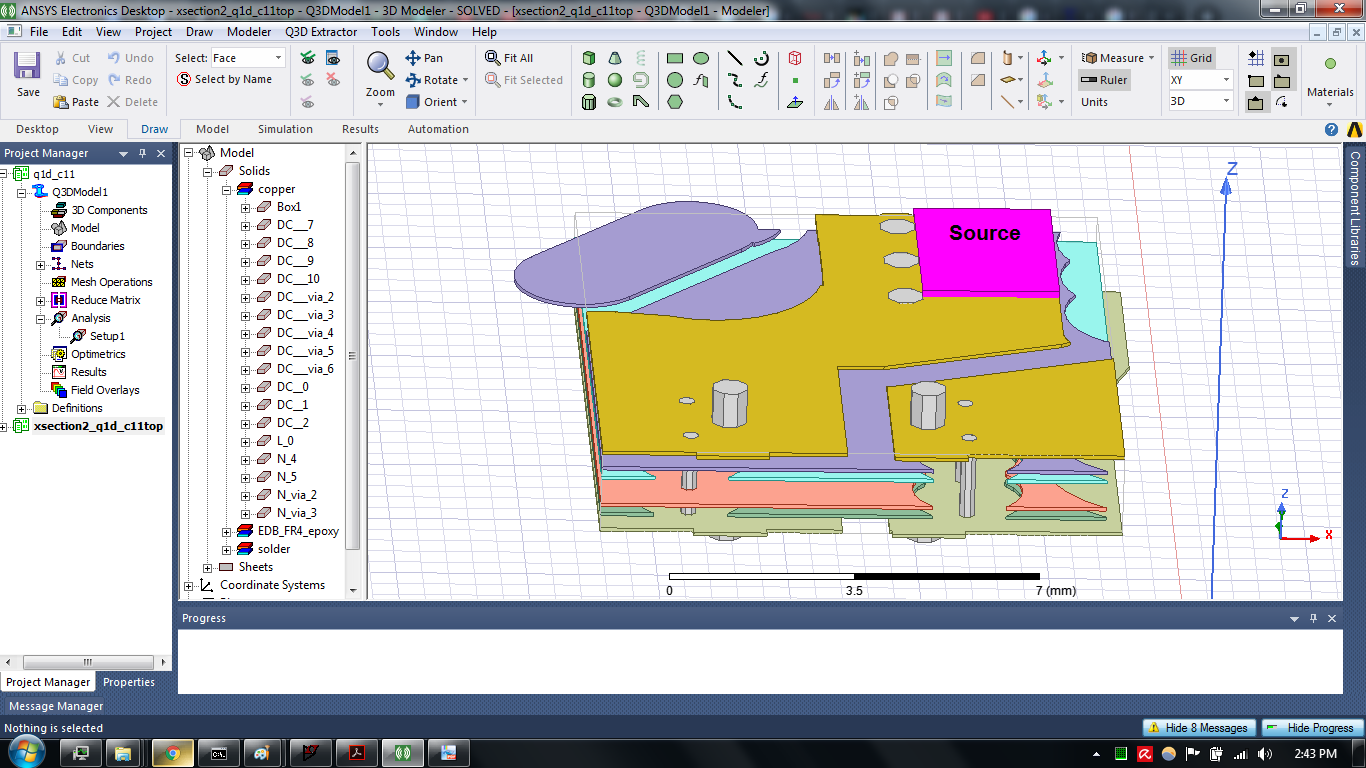
\includegraphics[width=\linewidth]{pictures/examples/Q1d_C11T_7.png}
  \caption{Q1-Drain sheet assigned as Source}
  \label{fig:source2}
\end{figure}

\begin{figure} [H]
  \centering
  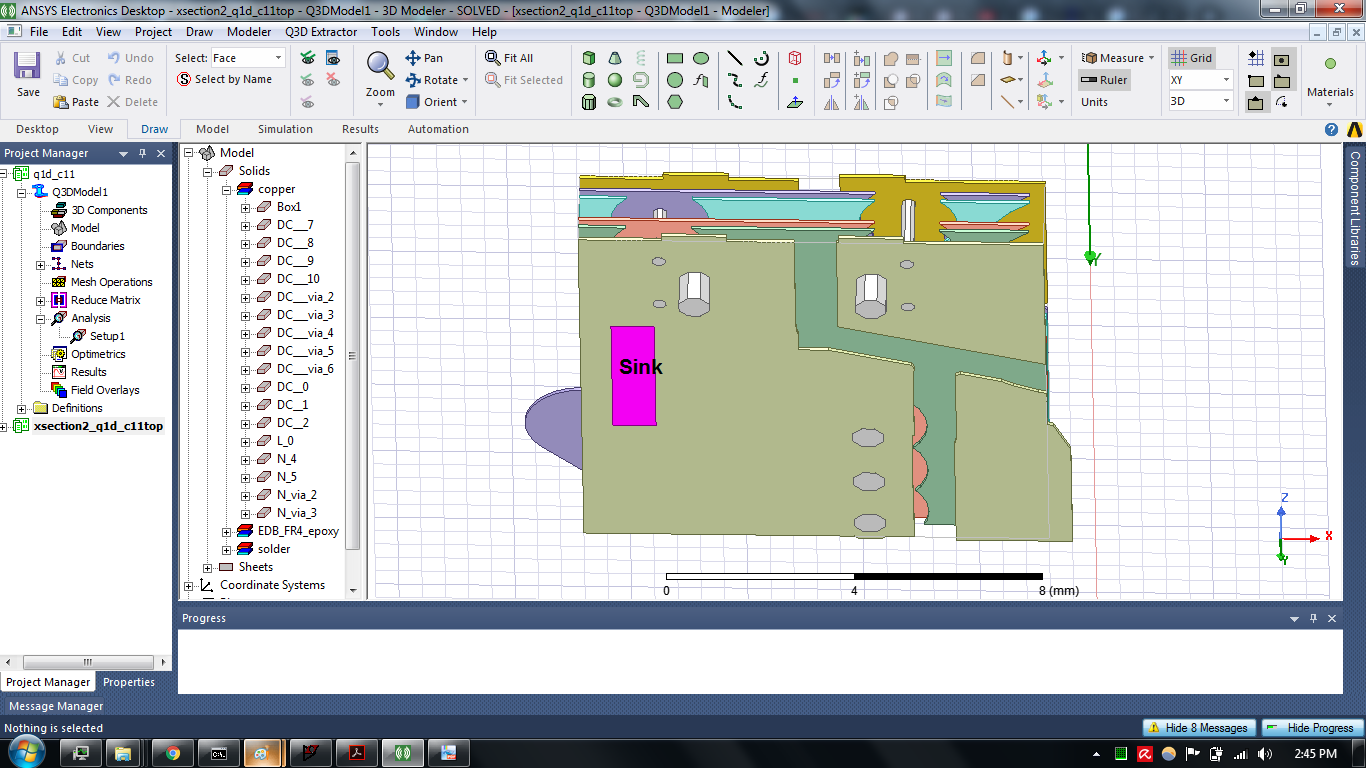
\includegraphics[width=\linewidth]{pictures/examples/Q1d_C11T_8.png}
  \caption{C11 sheet assigned as Sink}
  \label{fig:sink2}
\end{figure}

\item Next, 'Validation Check' is done prior to analysis to check for any errors with the design that might prevent the extraction process.

\begin{figure} [H]
  \centering
  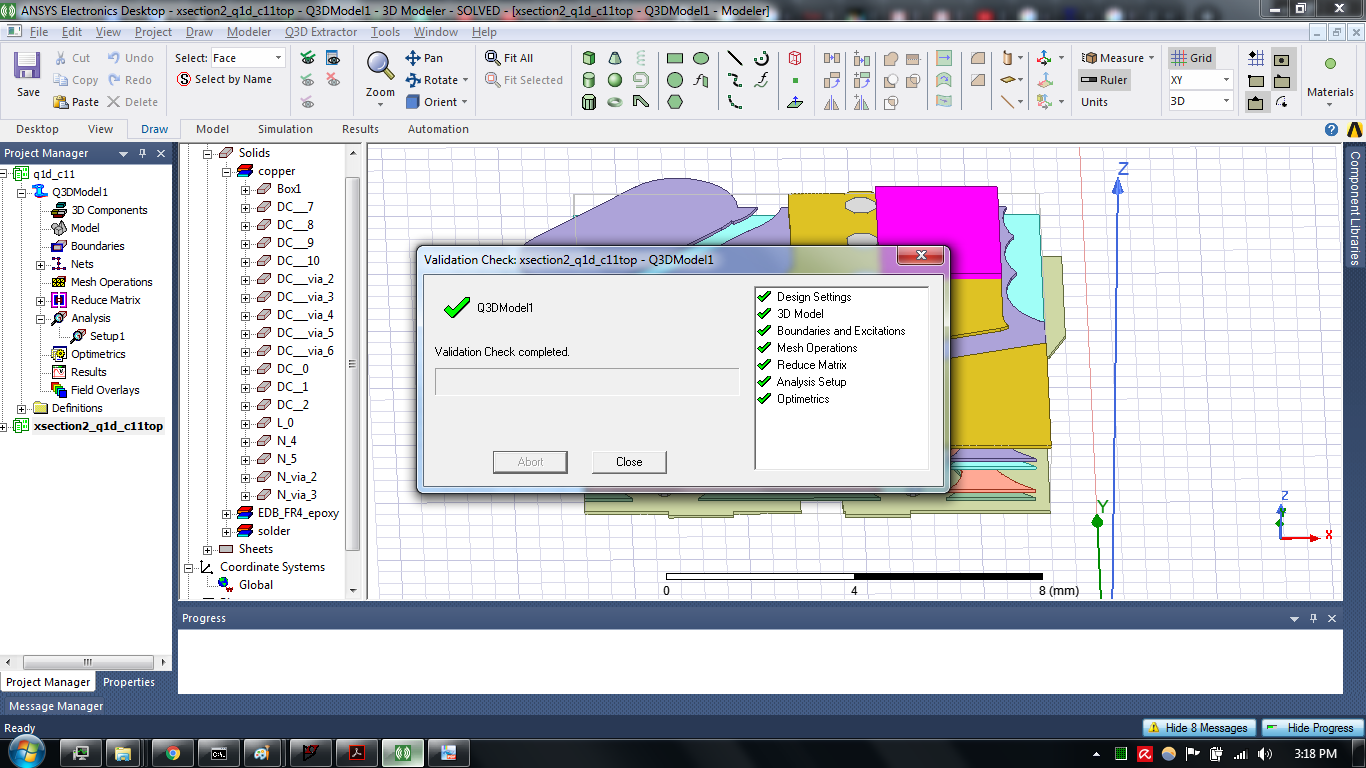
\includegraphics[width=\linewidth]{pictures/examples/valid.png}
  \caption{'Validation Check' returns no error}
  \label{fig:valid}
\end{figure}

\item Since 'Validation Check' returned no error, after adding 'Solution Setup', the final step 'Analysis' is carried out to extract the parasitic components

\begin{figure} [H]
  \centering
  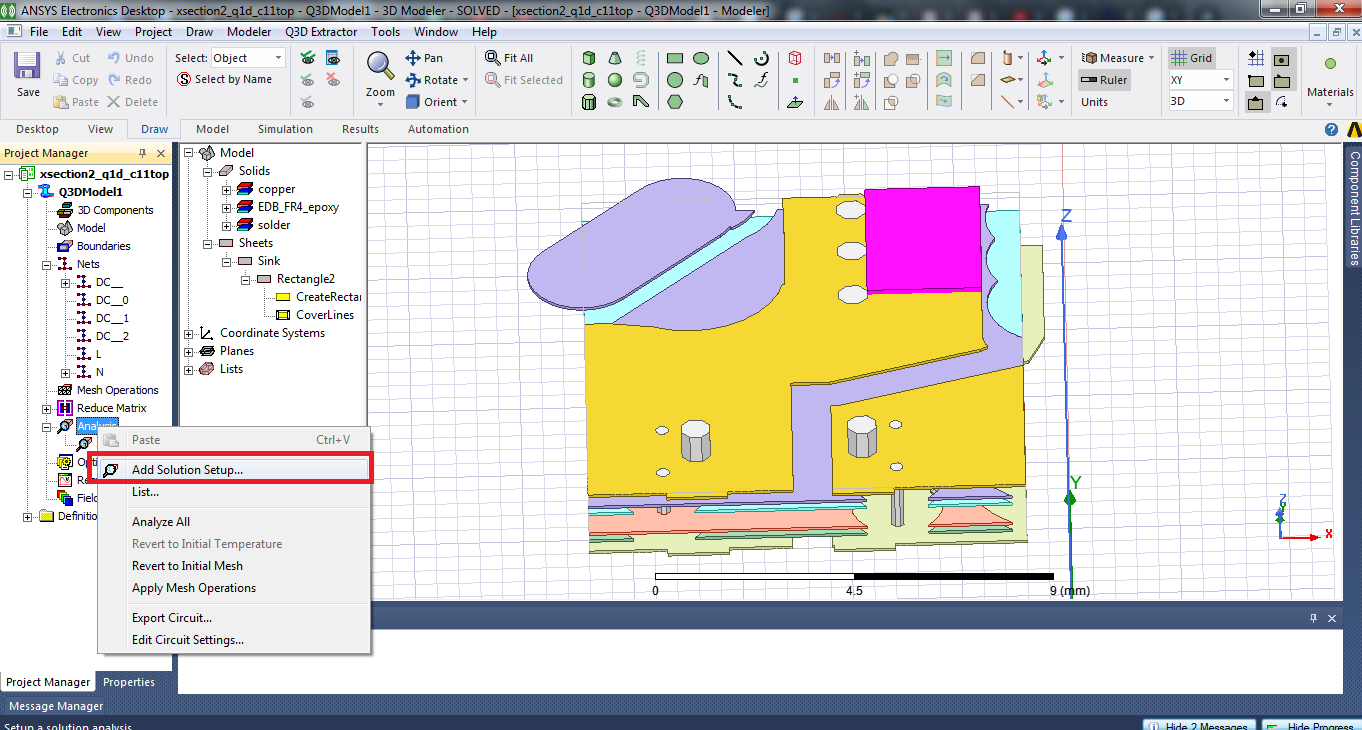
\includegraphics[width=\linewidth]{pictures/examples/solution.png}
  \caption{Add Solution Setup to configure the analysis requirements}
  \label{fig:solution}
\end{figure}

\begin{figure} [H]
  \centering
  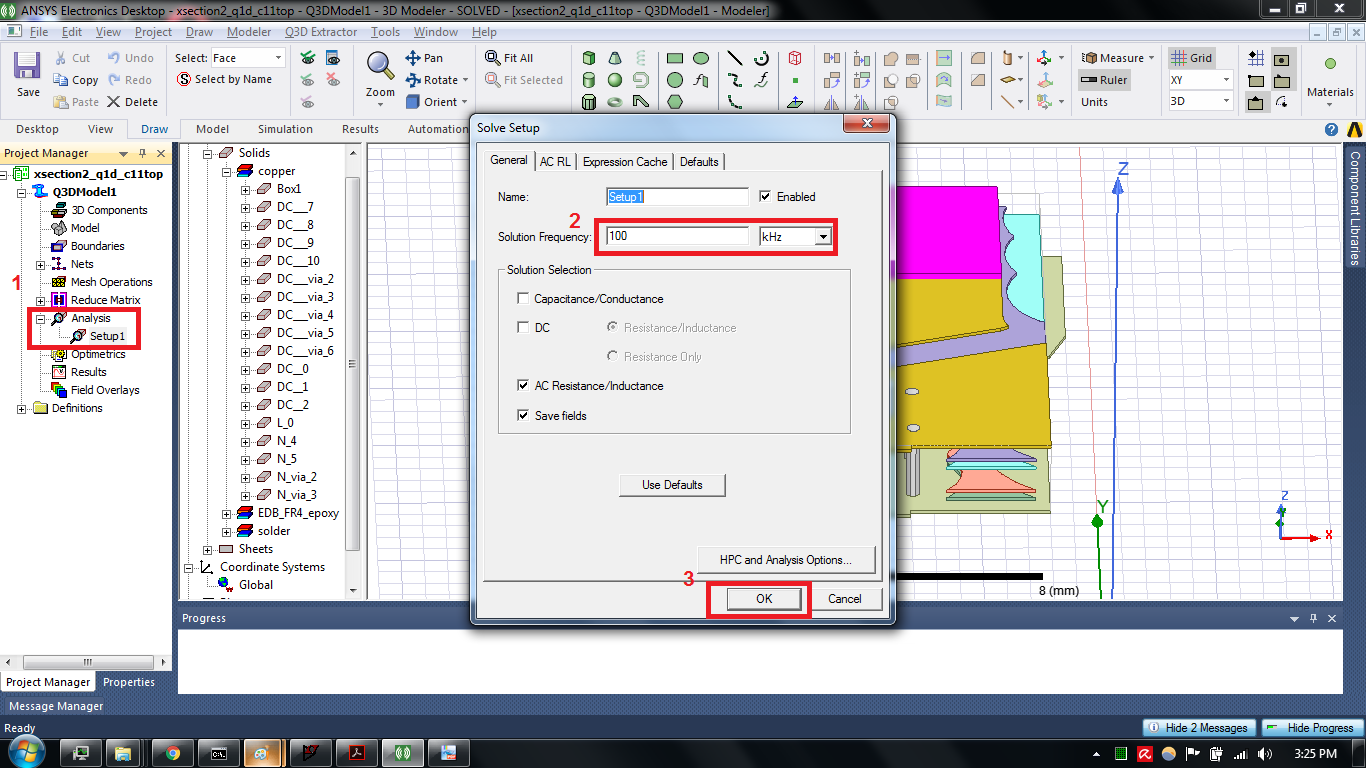
\includegraphics[width=\linewidth]{pictures/examples/setup.png}
  \caption{Analysis is configured through 'Add Solution Setup'}
  \label{fig:setup}
\end{figure}

\begin{figure} [H]
  \centering
  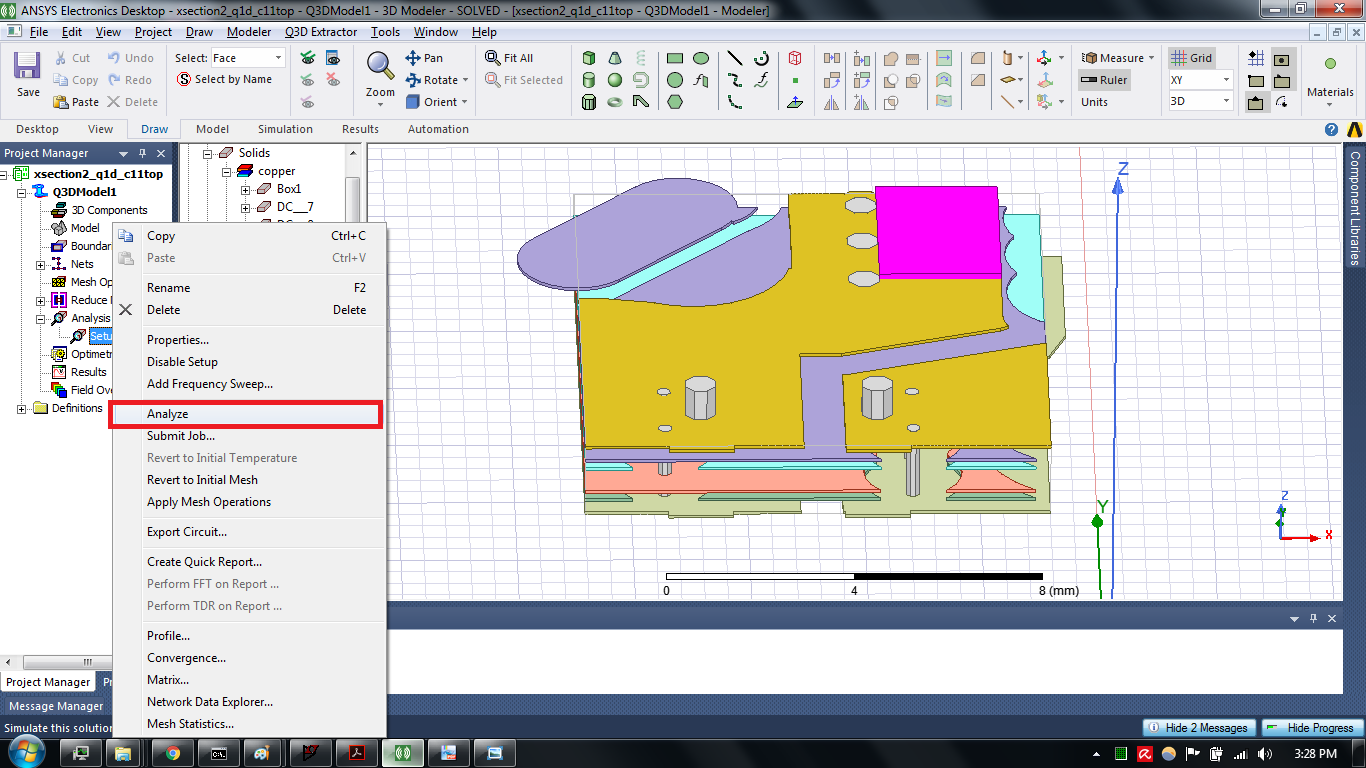
\includegraphics[width=\linewidth]{pictures/examples/analysis.png}
  \caption{Finally 'Analyze' is done}
  \label{fig:setup}
\end{figure}

\begin{figure} [H]
  \centering
  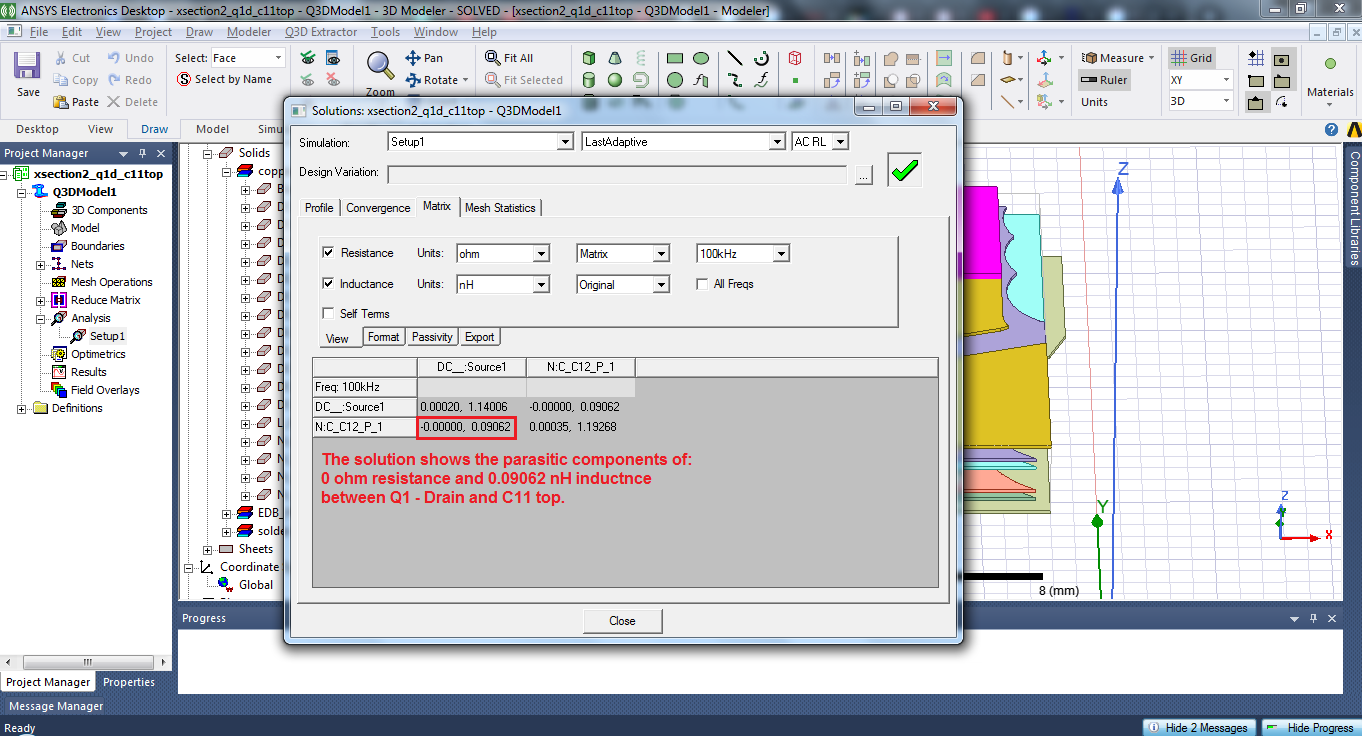
\includegraphics[width=\linewidth]{pictures/examples/results.png}
  \caption{Solution showing the parasitic components}
  \label{fig:results}
\end{figure}

\item In the end, the extracted parasitic components are collected and added to the SPICE model. Parasitic components from other branches of the circuit are extracted using similar method and when all the branches are solved, analysis is done on the SPICE model to compare the ideal model (without the parasitic components) and the extracted model (with the parasitic components)

\begin{figure} [H]
  \centering
  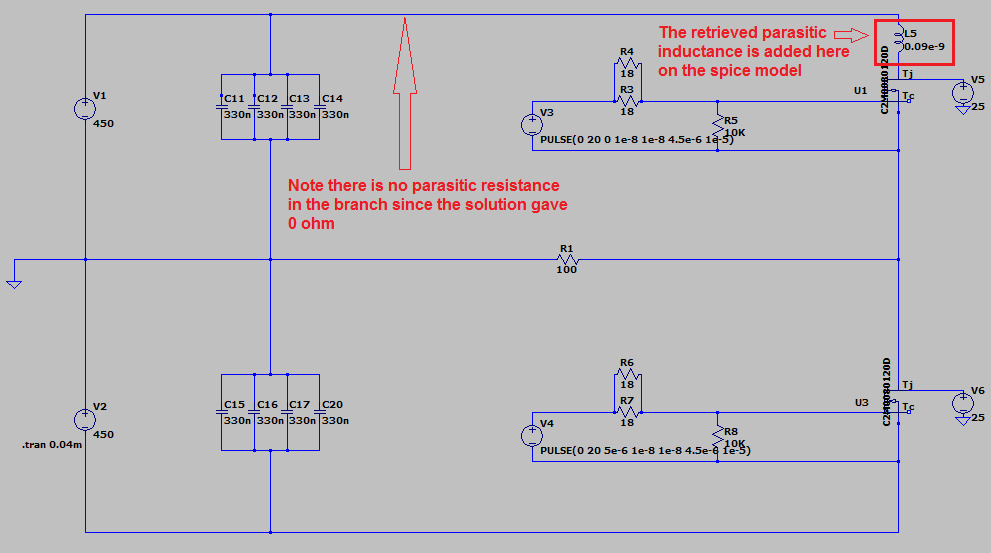
\includegraphics[width=\linewidth]{pictures/examples/spice2.png}
  \caption{Parasitic inductance added to the SPICE model}
  \label{fig:results}
\end{figure}

\end{enumerate}

\subsubsection{Other examples of extracting parasitic inductance and resistance}
\label{sec:other_ind_res}

The images below gives two more examples showing how ANSYS was used to harvest the parasitic information between 2 branches of the circuit.

\subsubsection{Extraction between Q3-Source and C16 in the DC- Net}
\label{sec:extraction_q3s_c16}

In the schematic, this is the part from where the parasitic is extracted.

\begin{figure} [H]
  \centering
  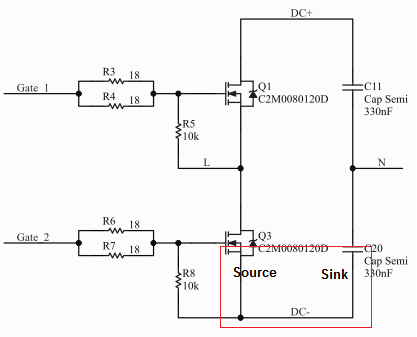
\includegraphics[width=\linewidth]{pictures/examples/schematic2.png}
  \caption{The red box indicates the portion from where parasitic is extracted}
  \label{fig:schematic2}
\end{figure}

\begin{figure} [H]
  \centering
  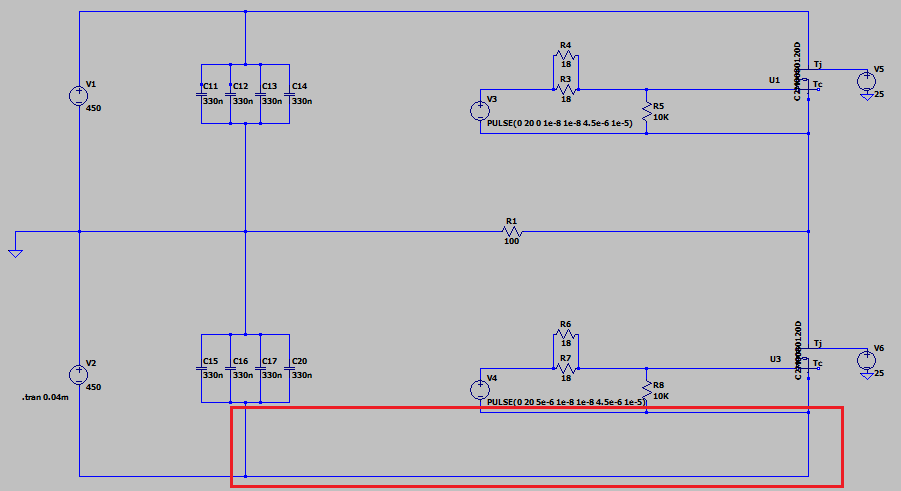
\includegraphics[width=\linewidth]{pictures/examples/spice3.png}
  \caption{The red box indicates the portion where the extracted parasitic is to be placed}
  \label{fig:spice3}
\end{figure}

From the PCB layout, if we ignore all other parts except the Net and the areas from where the parasitic is extracted, the layout looks like the following

\begin{figure} [H]
  \centering
  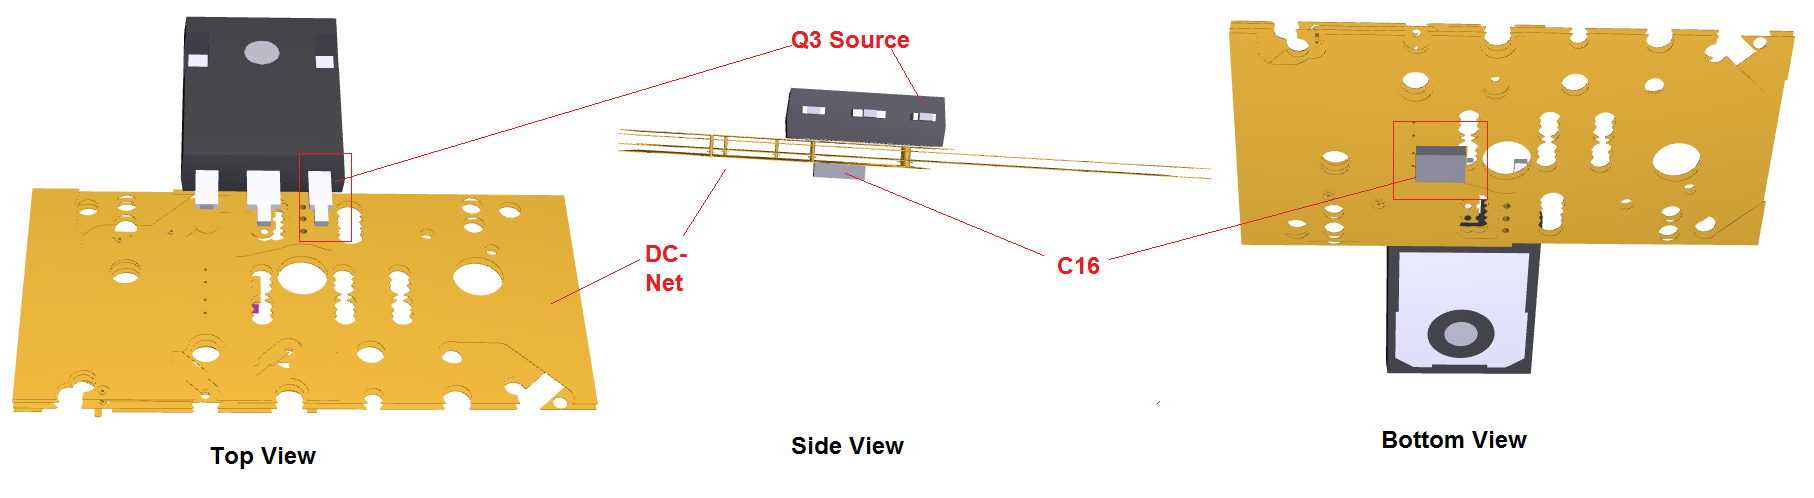
\includegraphics[width=\linewidth]{pictures/examples/PCB_cut2.png}
  \caption{Portion of PCB that is of concern}
  \label{fig:PCB_cut2}
\end{figure}

In ANSYS Q3D, we analyze the PCB part to find the parasitic components

\begin{figure} [H]
  \centering
  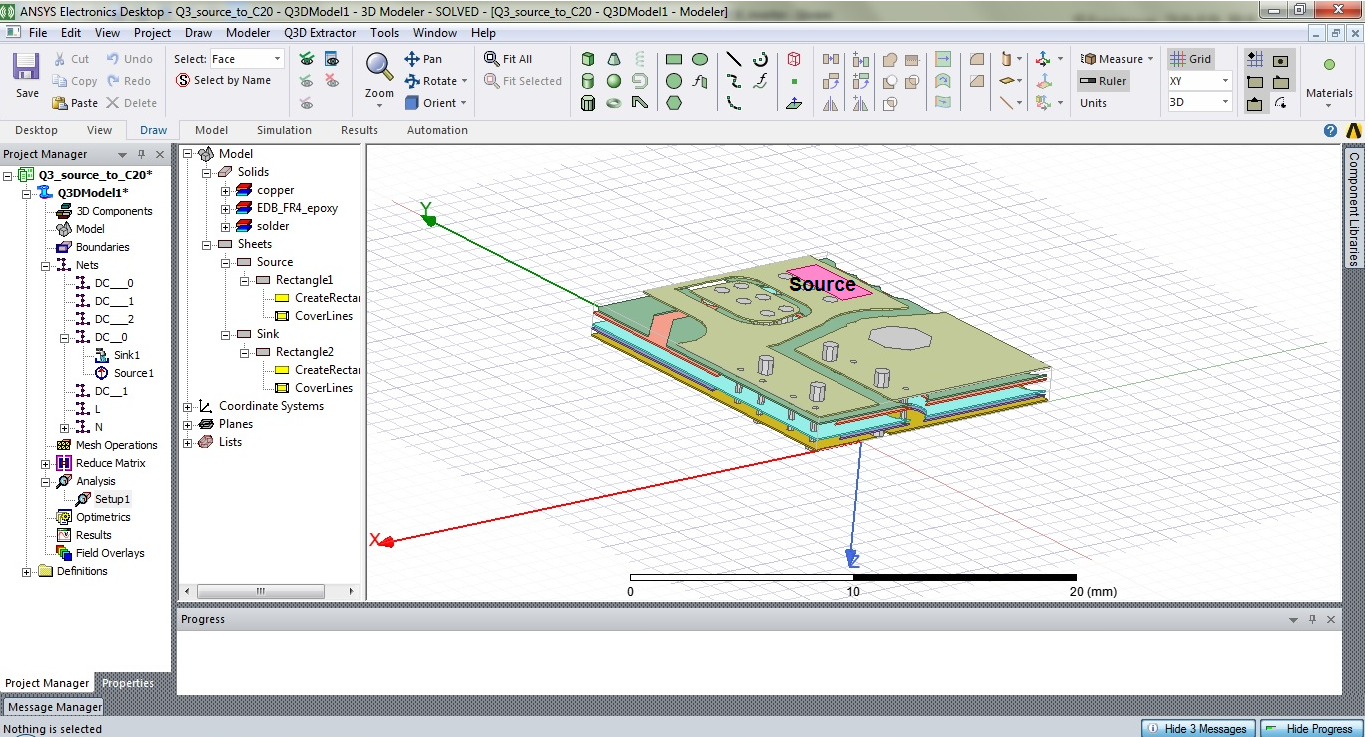
\includegraphics[width=\linewidth]{pictures/examples/Q3S_C16_Source.png}
  \caption{Marking the Source position at Q3-Source in the DC- Net}
  \label{fig:Q3s_C16_source}
\end{figure}

\begin{figure} [H]
  \centering
  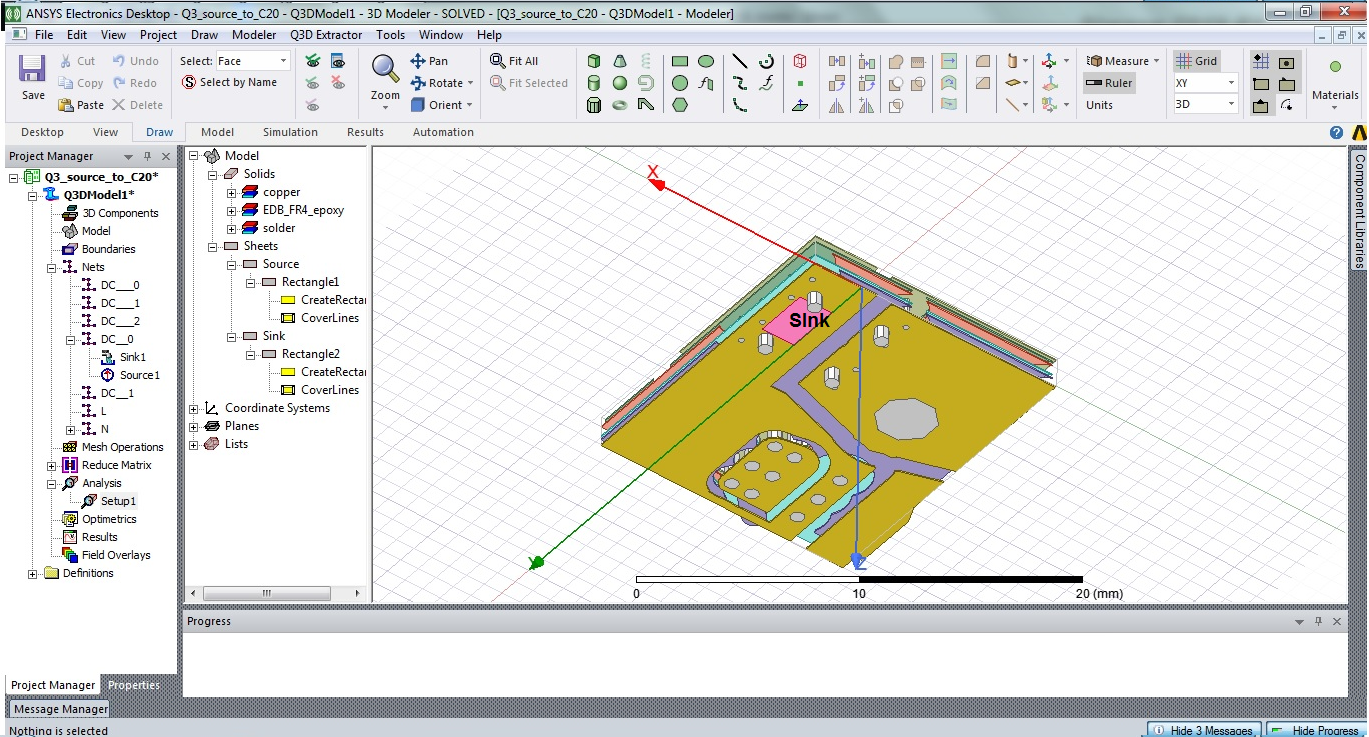
\includegraphics[width=\linewidth]{pictures/examples/Q3S_C16_Sink.png}
  \caption{Marking the Sink position at C16 in the DC- Net}
  \label{fig:Q3s_C16_sink}
\end{figure}

\begin{figure} [H]
  \centering
  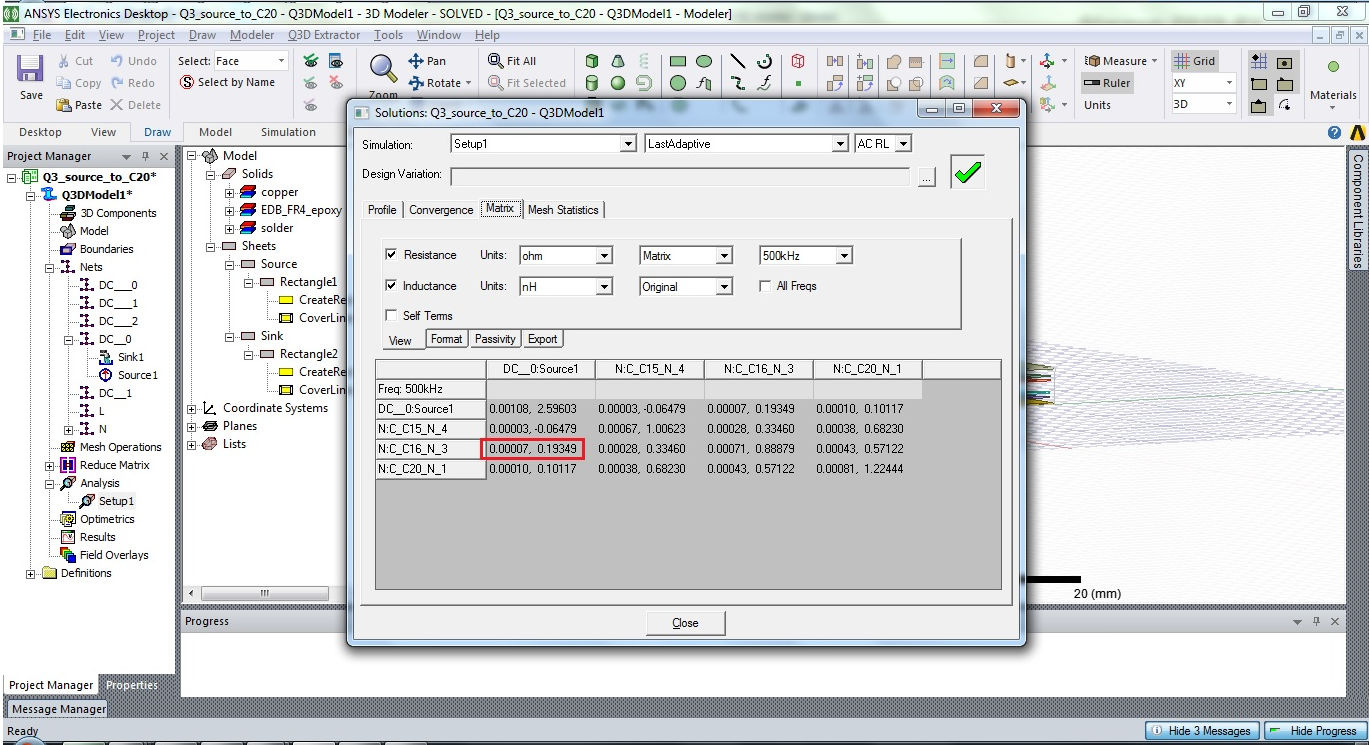
\includegraphics[width=\linewidth]{pictures/examples/Q3S_C16_extractions.png}
  \caption{Extracted parasitic components}
  \label{fig:Q33_C16_extractions}
\end{figure}

\subsubsection{Extraction between C11 and C20 in the N Net}
\label{sec:extraction_c11_c20}

In the schematic, this is the part from where the parasitic is extracted

\begin{figure} [H]
  \centering
  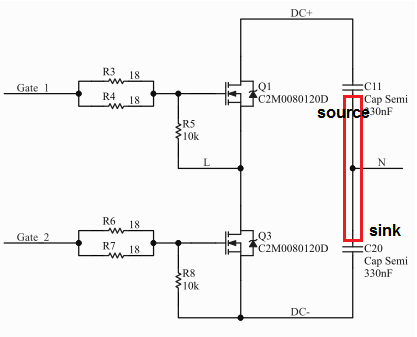
\includegraphics[width=\linewidth]{pictures/examples/schematic3.png}
  \caption{The red box indicates the portion from where parasitic is extracted}
  \label{fig:schematic3}
\end{figure}

From the PCB layout, if we ignore all other parts except the Net and the areas from where the parasitic is extracted, the layout looks like the following.

\begin{figure} [H]
  \centering
  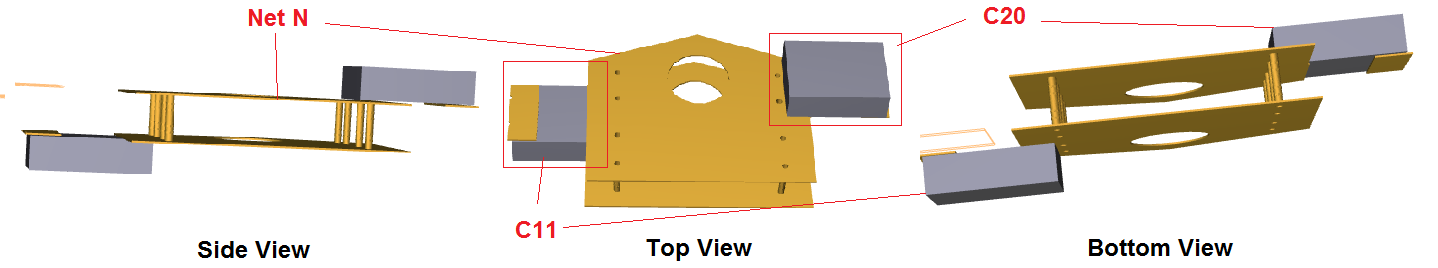
\includegraphics[width=\linewidth]{pictures/examples/PCB_cut_3.png}
  \caption{Portion of PCB that is of concern}
  \label{fig:PCB_cut3}
\end{figure}

\begin{figure} [H]
  \centering
  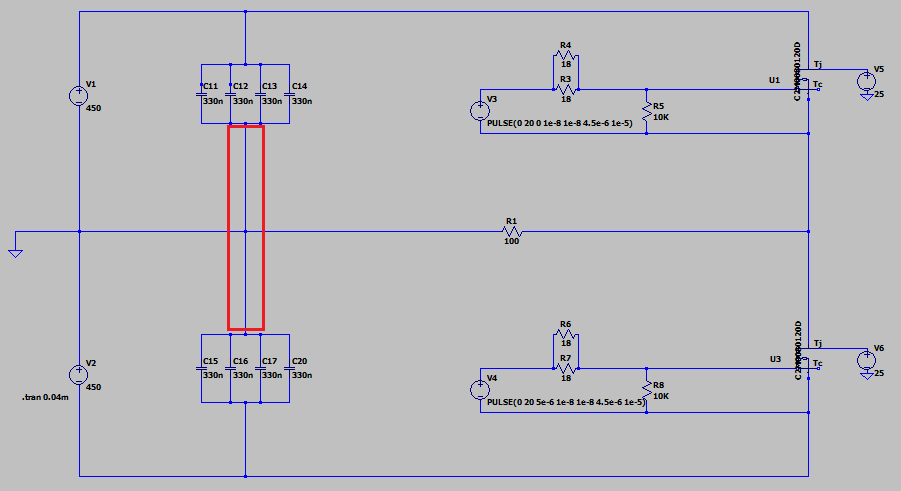
\includegraphics[width=\linewidth]{pictures/examples/spice4.png}
  \caption{The red box indicates the portion where the extracted parasitic is to be placed}
  \label{fig:spice4}
\end{figure}

In ANSYS Q3D, we analyze the PCB part to find the parasitic components.

\begin{figure} [H]
  \centering
  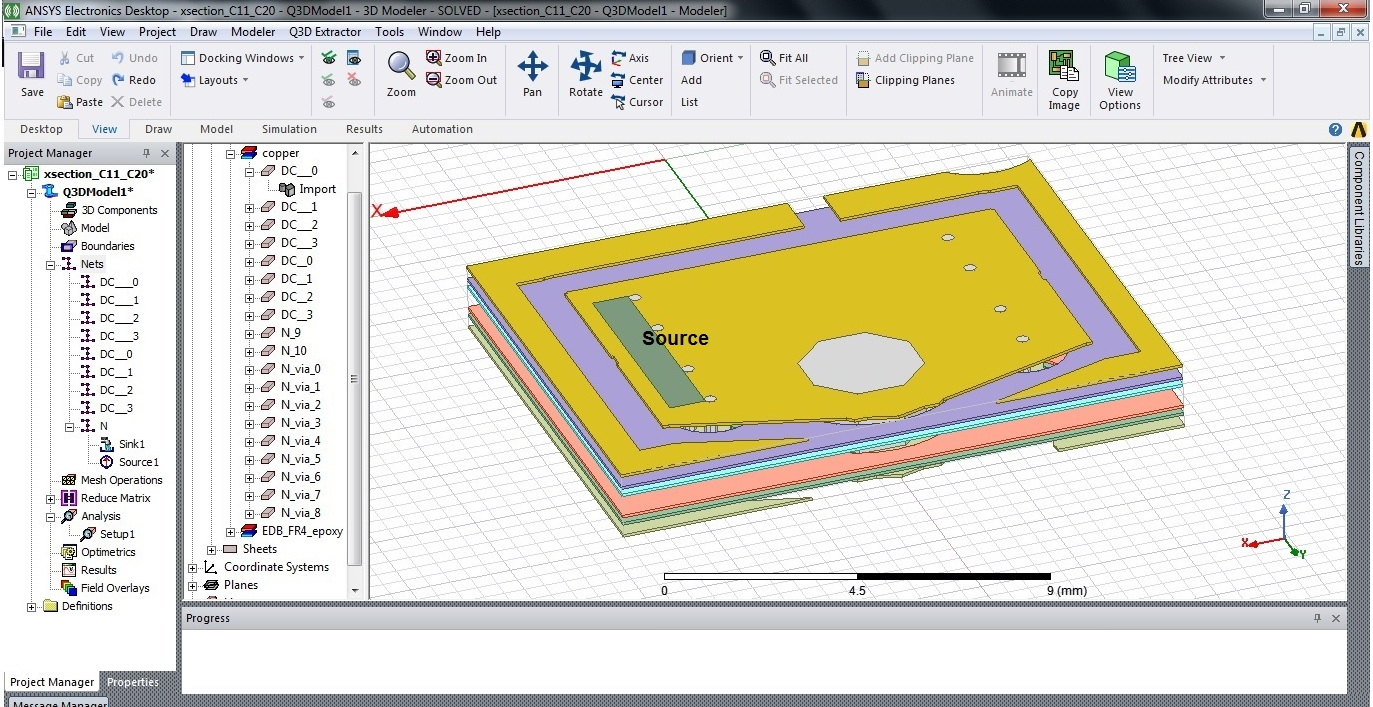
\includegraphics[width=\linewidth]{pictures/examples/c11_c20_source.png}
  \caption{Marking the Source position at C11 in the N Net}
  \label{fig:C11_C20_source}
\end{figure}

\begin{figure} [H]
  \centering
  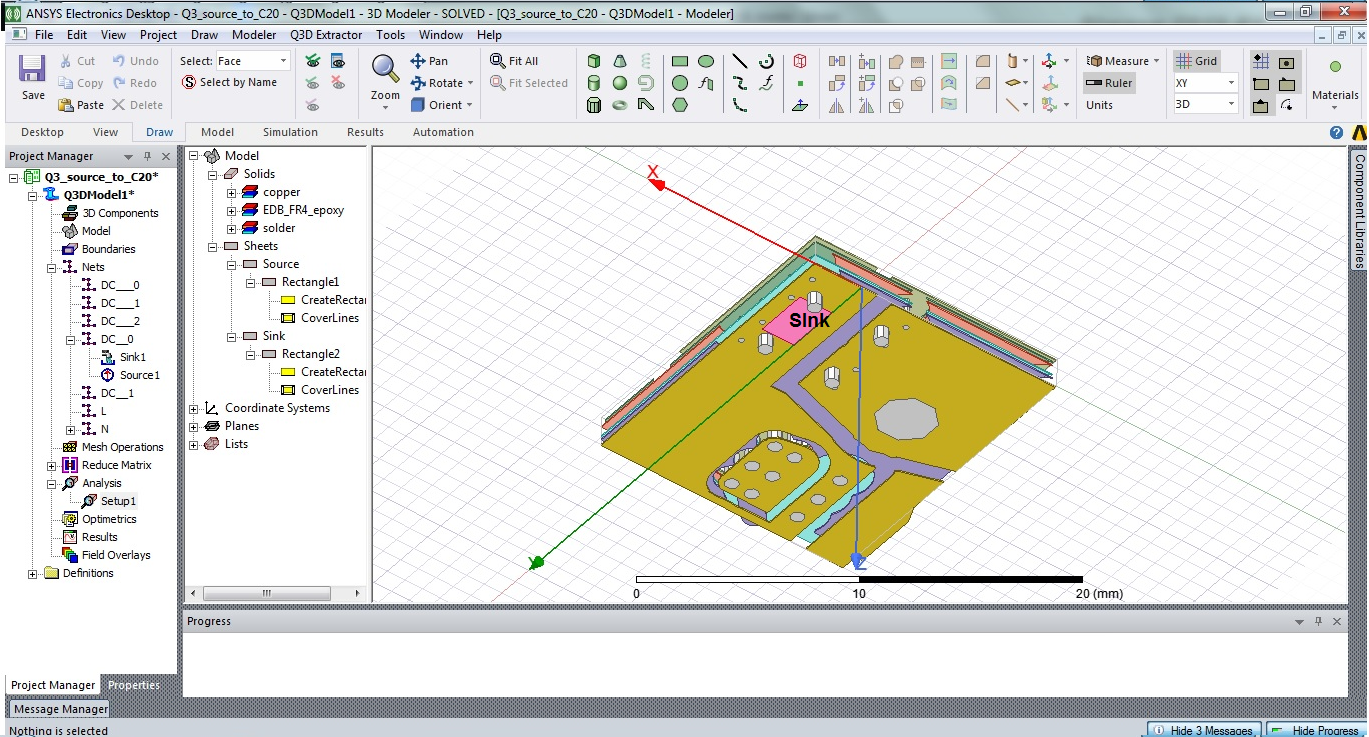
\includegraphics[width=\linewidth]{pictures/examples/Q3S_C16_Sink.png}
  \caption{Marking the Sink position at C20 in the N Net}
  \label{fig:C11_C20_sink}
\end{figure}

\begin{figure} [H]
  \centering
  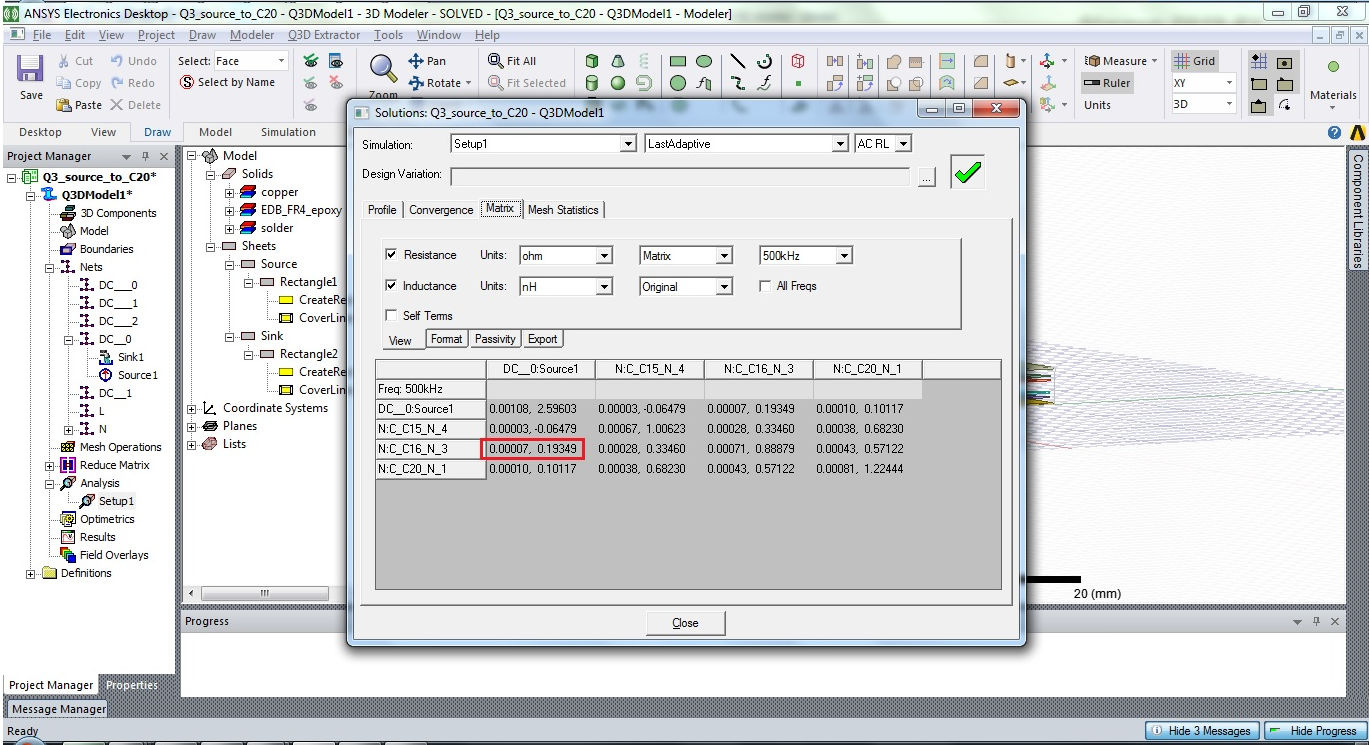
\includegraphics[width=\linewidth]{pictures/examples/Q3S_C16_extractions.png}
  \caption{Extracted parasitic components}
  \label{fig:C11_C20_extractions}
\end{figure}

\subsubsection{Step-by-step extraction process for parasitic capacitance between Q1-Gate and Q1-Drain}

The exact same procedure mentioned in Section 6.6.2 Step 1 - 6 is followed. From Step 7, extracting parasitic capacitance differs from how parasitic inductance and resistance is retrieved.

\begin{enumerate}

\item First, we need to target from the schematic:

\begin{figure} [H]
  \centering
  \includegraphics[width=\linewidth]{pictures/examples/Schematic5.png}
  \caption{The red box indicates the portion from where parasitic is extracted}
  \label{fig:schematic5}
\end{figure}

\item  The target is also marked in the corresponding SPICE model since the extracted parasitic components will be included between these particular branches.

\begin{figure} [H]
  \centering
  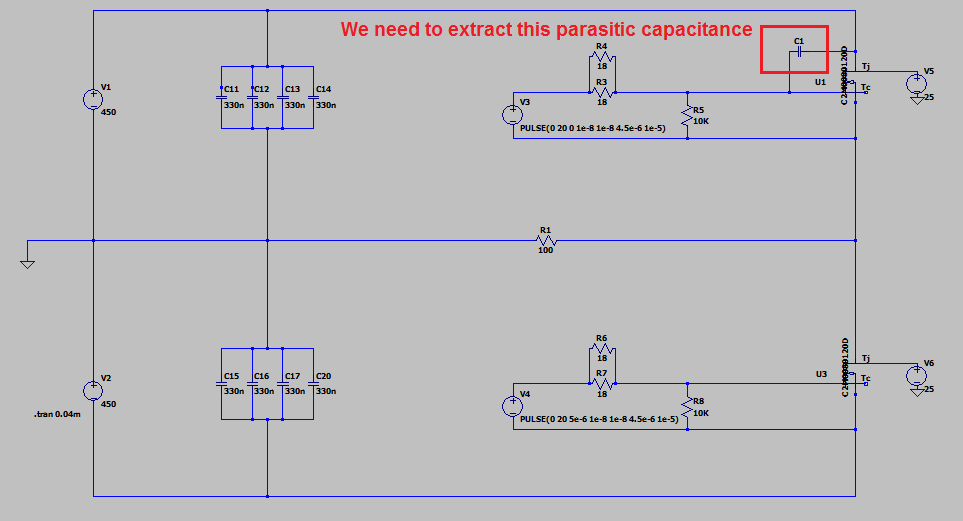
\includegraphics[width=\linewidth]{pictures/examples/spice5.png}
  \caption{The red box indicates the portion where the extracted parasitic is to be placed}
  \label{fig:spice5}
\end{figure}

\item From the PDF PCB layout, if all other components are ignored  except the Net DC+ (which contains the Q1-drain) and the net Q1-Gate from where the parasitic components are extracted, the layout looks like the following.

\begin{figure} [H]
  \centering
  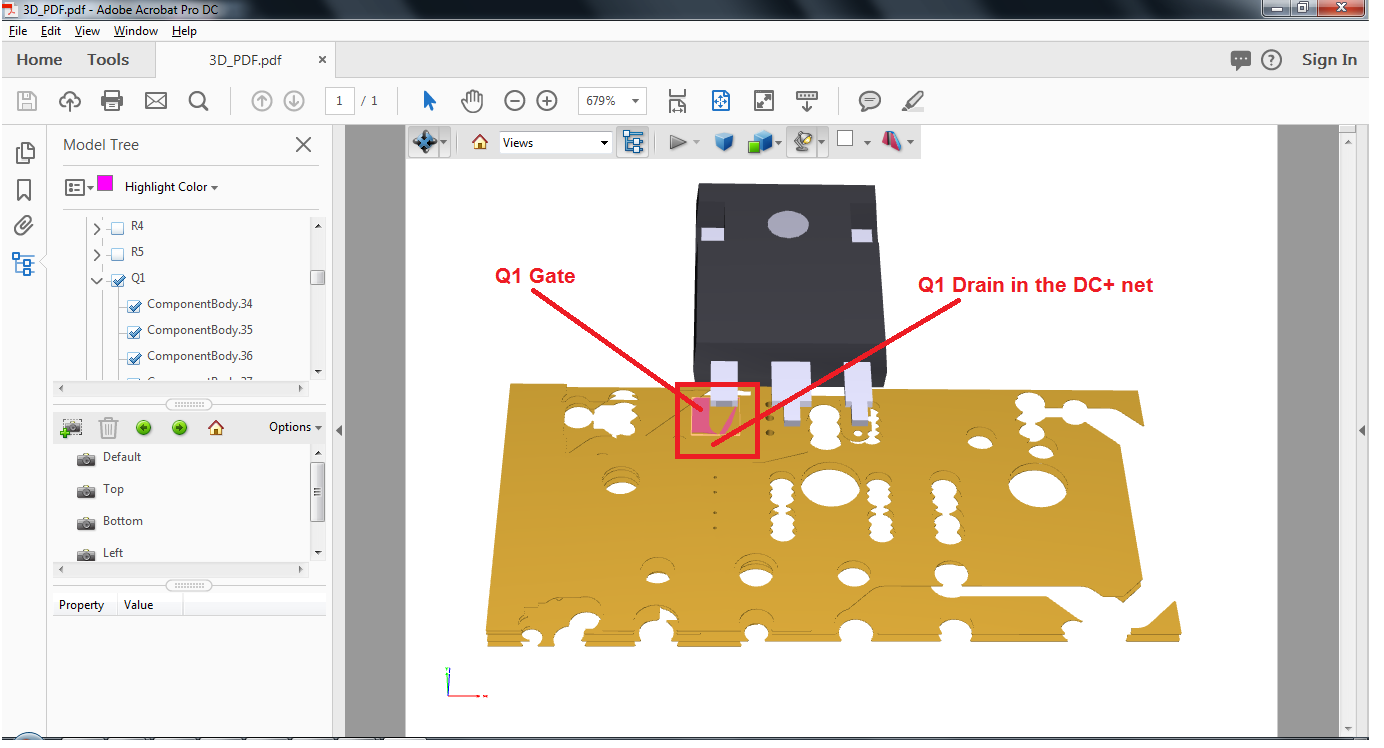
\includegraphics[width=\linewidth]{pictures/examples/PCB_cut_4.png}
  \caption{Portion of PCB that is of concern}
  \label{fig:PCB_cut4}
\end{figure}

\item Next, the PDF graphics layout is used to identify the part of interest where both the nets DC+ (containing Q1-Drain) and Q1-gate overlaps. Then, the same area is located in the ANSYS SIwave 3D PCB layout and that portion is clipped.

\begin{figure} [H]
  \centering
  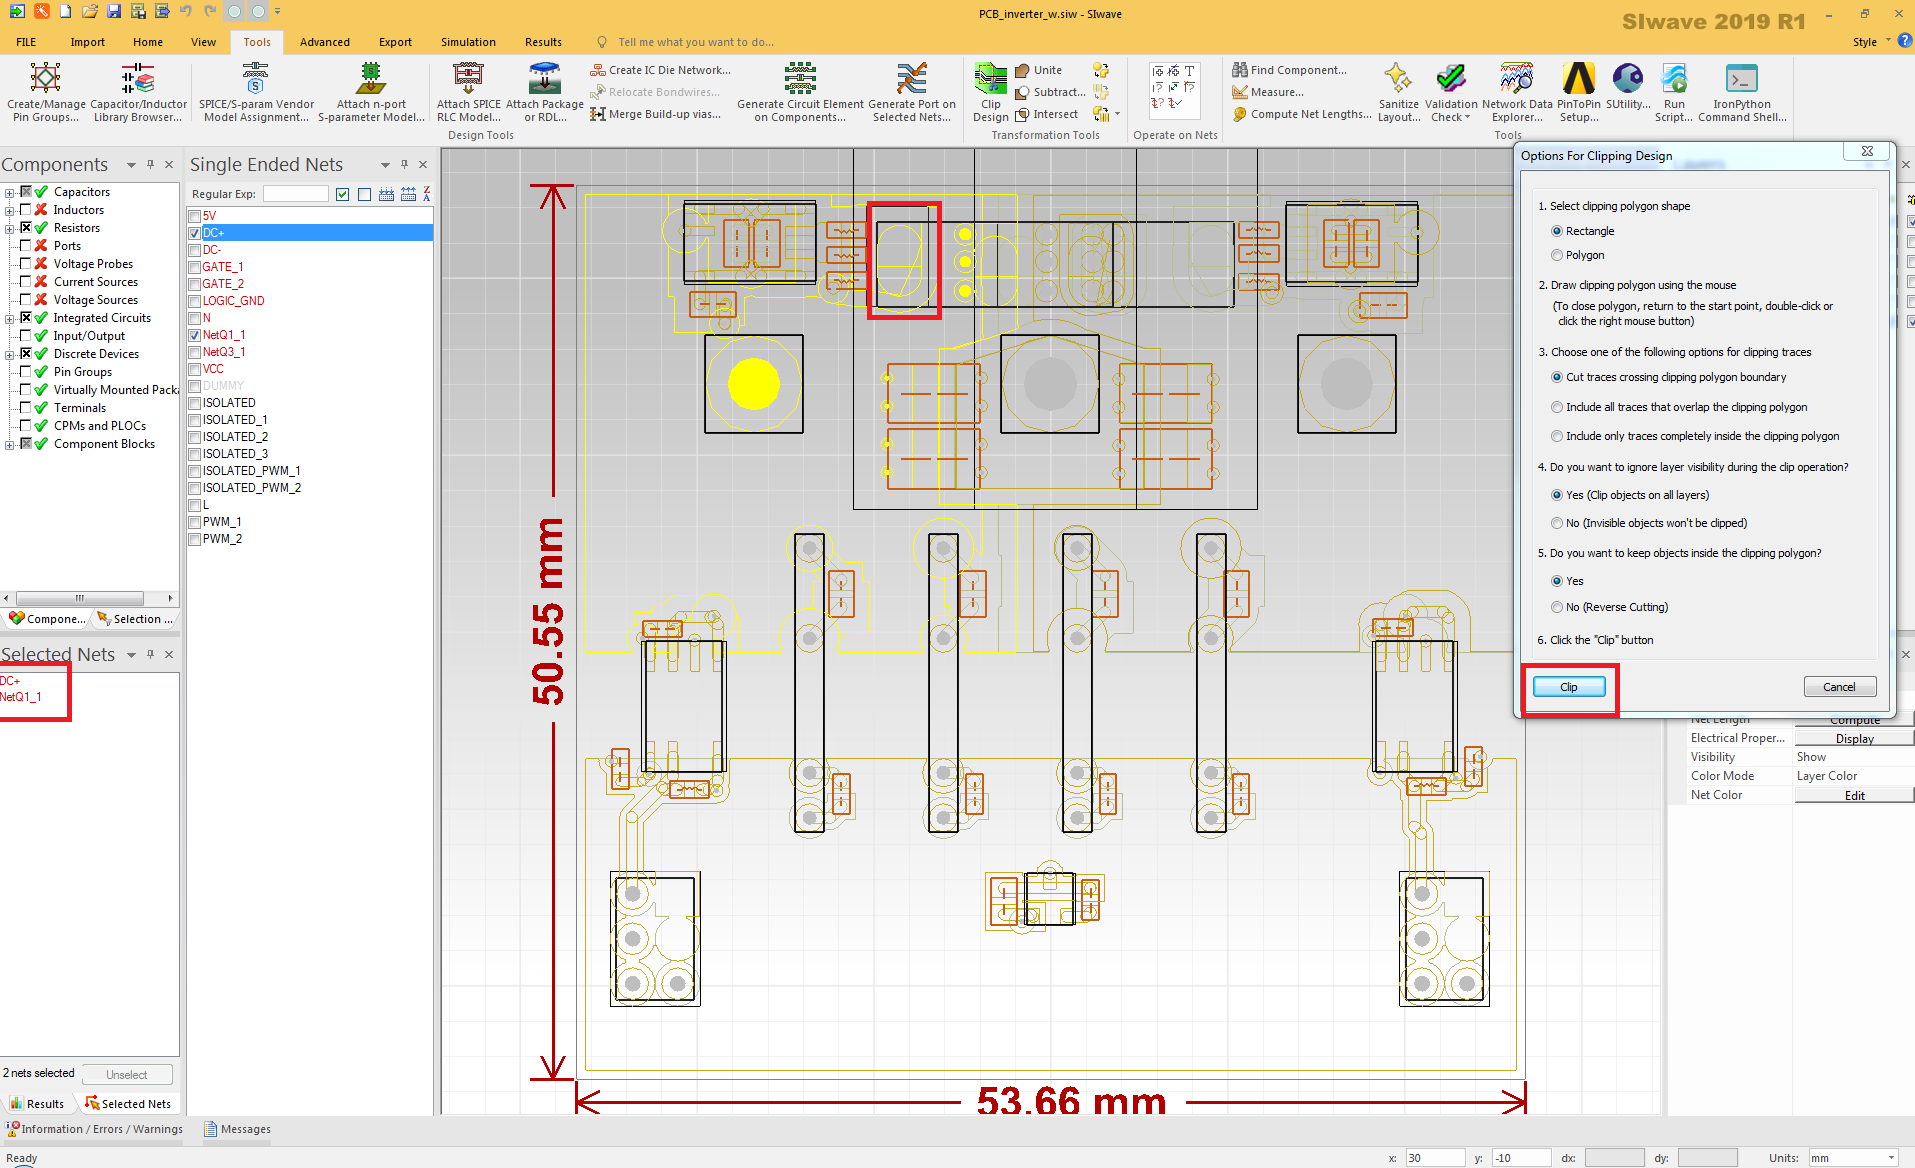
\includegraphics[width=\linewidth]{pictures/examples/siwave_td2.png}
  \caption{Identifying overlapped area of Q1-Gate and Q1-Drain from top-down view}
  \label{fig:PCB_identify2}
\end{figure}

\begin{figure} [H]
  \centering
  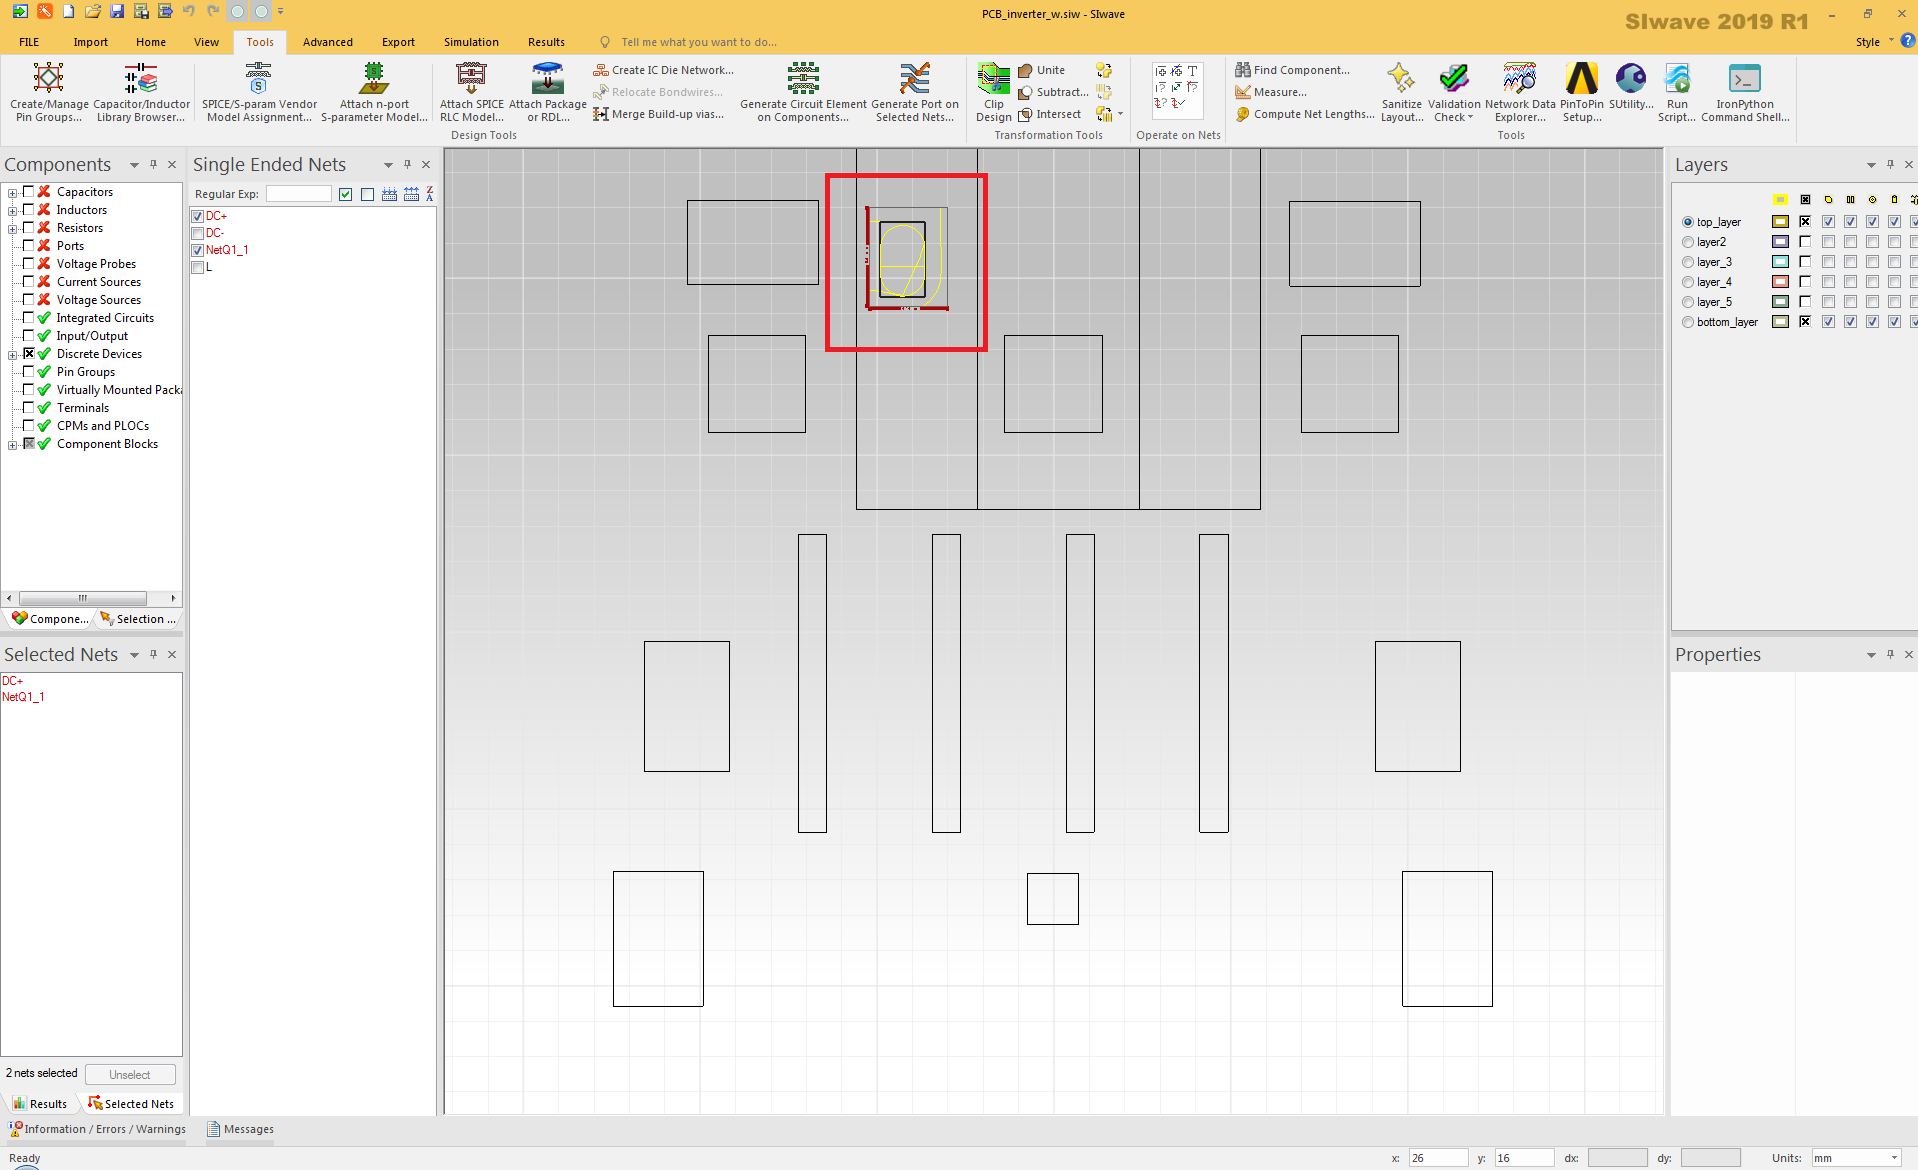
\includegraphics[width=\linewidth]{pictures/examples/siwave_clip3.png}
  \caption{Clipped Portion of PCB that is of concern containing the overlapped nets of Q1-Drain and Q1-Source}
  \label{fig:PCB_clip3}
\end{figure}

\item The clipped portion is properly checked and verified to contain the part of interest. Repeat step 4 if clipping seems to have an error.

\begin{figure} [H]
  \centering
  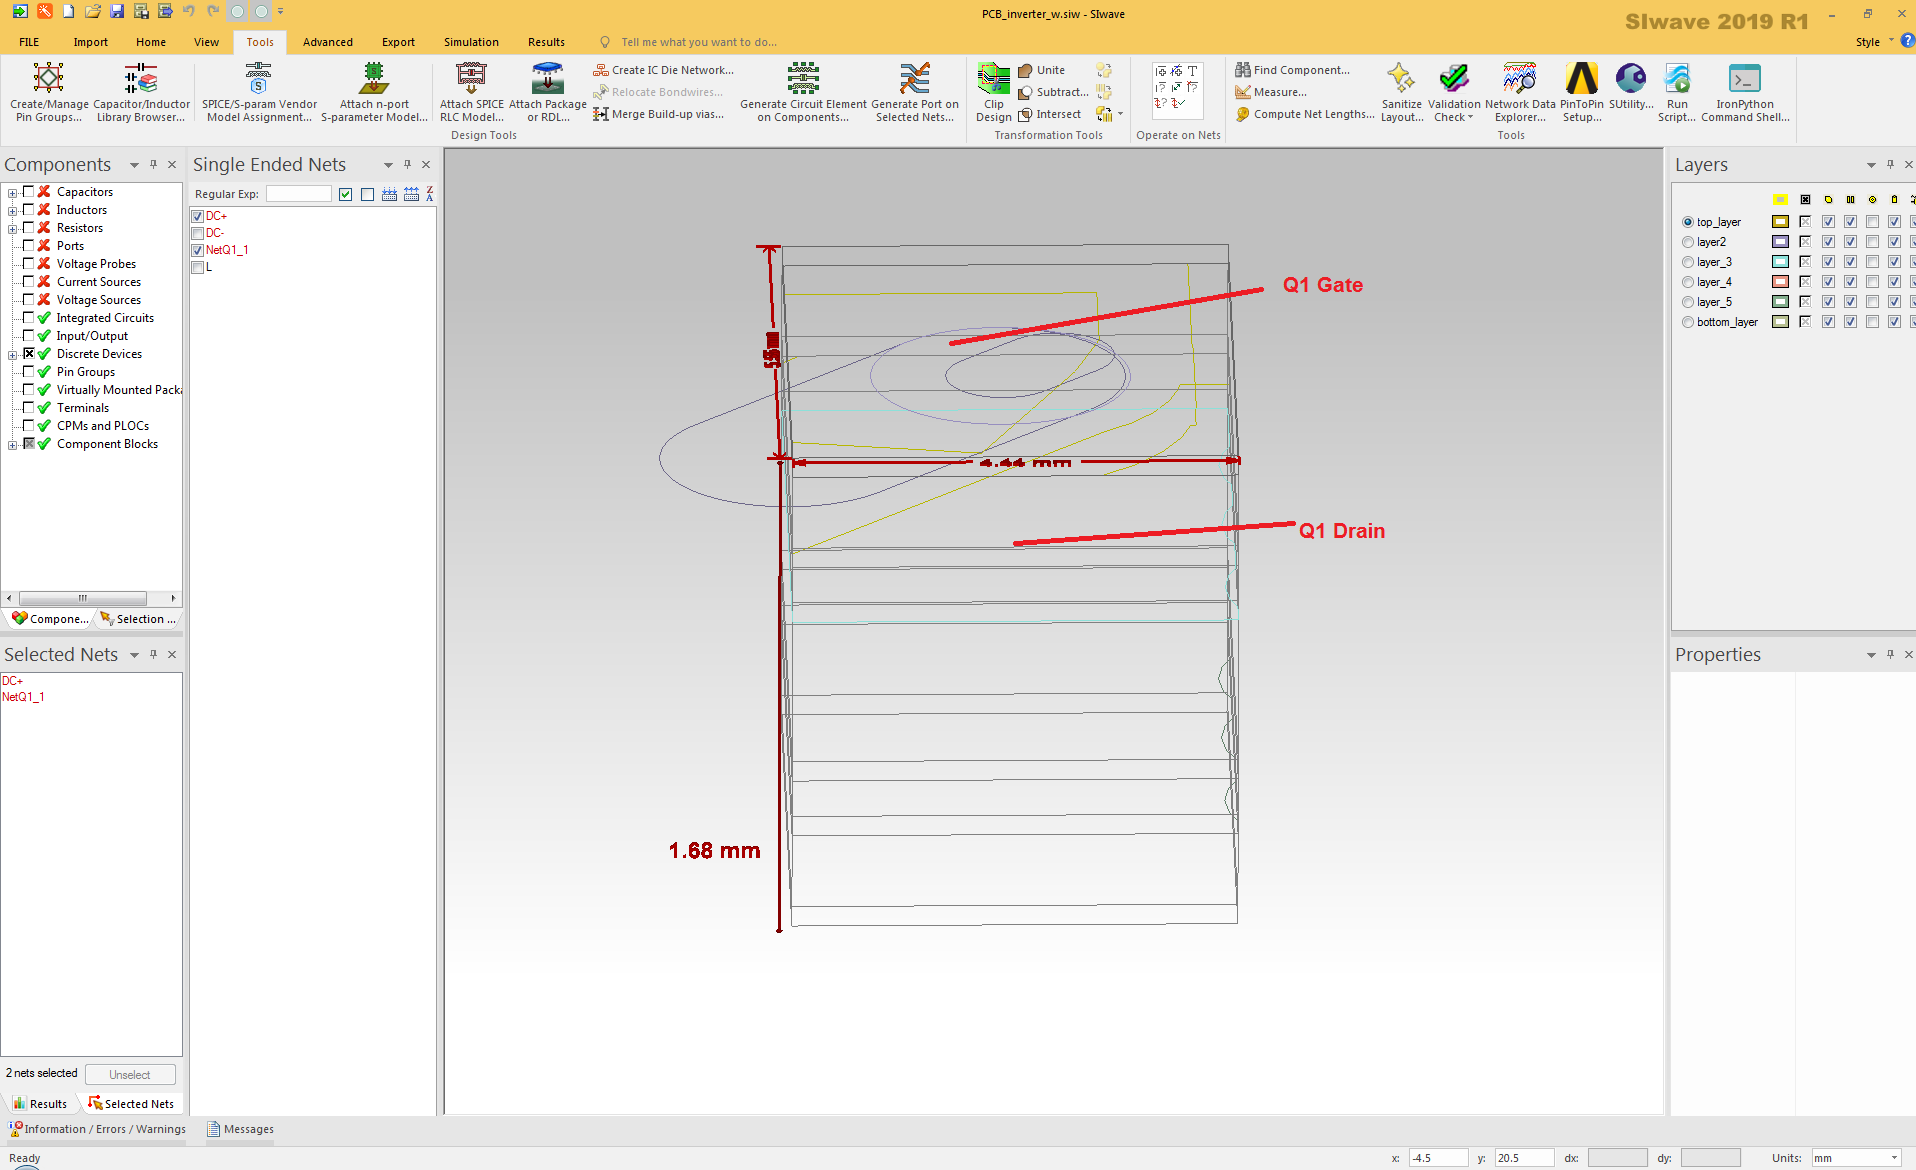
\includegraphics[width=\linewidth]{pictures/examples/siwave_verified.png}
  \caption{Verifying the clipped part of the original PCB layout}
  \label{fig:PCB_verified2}
\end{figure}

\item The clipped portion is exported to ANSYS Q3D Extractor to extract the parasitic components.

\begin{figure} [H]
  \centering
  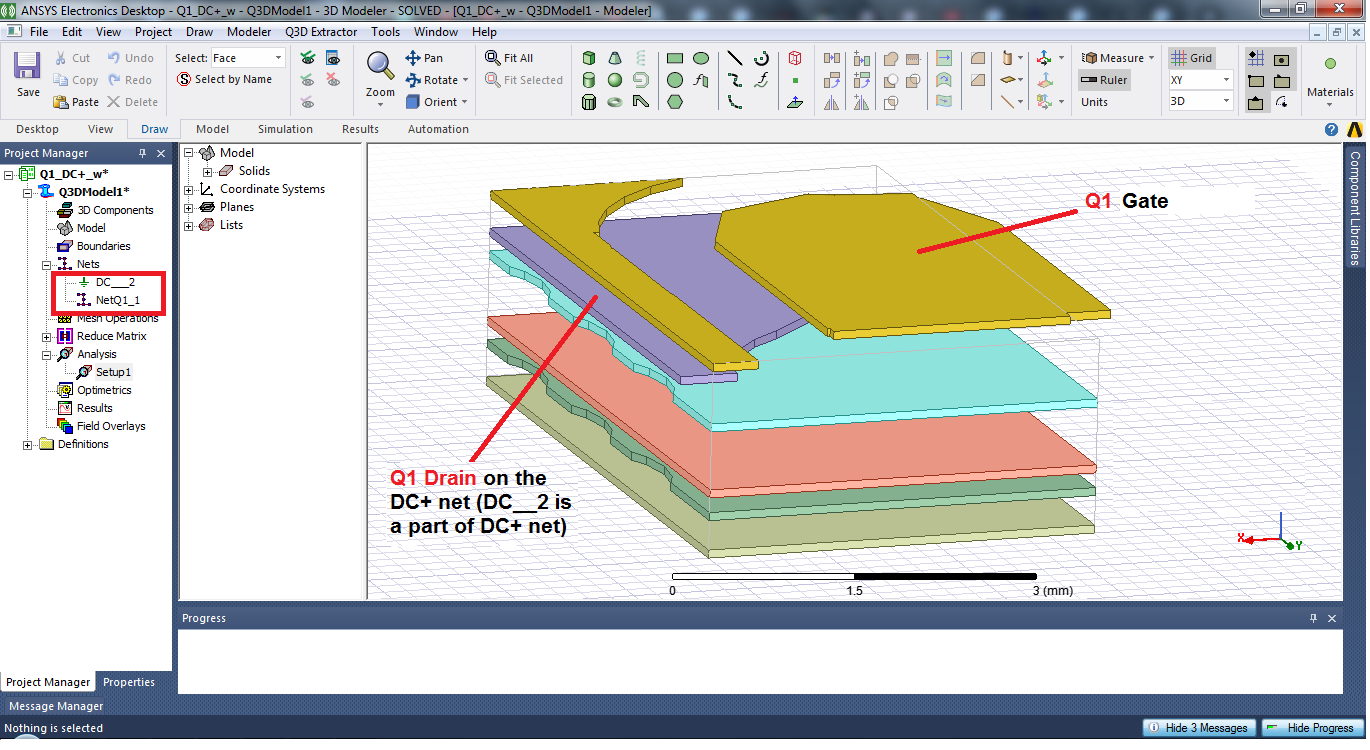
\includegraphics[width=\linewidth]{pictures/examples/cap_q1_g_d}
  \caption{Clipped PCB part is exported to ANSYS Q3D}
  \label{fig:cap_q1_g_d}
\end{figure}

\item In ANSYS Q3D, the clipped PCB part where the Q1 gate and drain overlap is analyzed to recover the parasitic components.\\

To find the parasitic components, we need to:
\begin{enumerate}
\item Make one of them Signal - Here, Q1 gate is assigned Signal 
\item The one of then Ground - Here, Q1 drain (in the DC+ net) is assigned Ground 
\end{enumerate}

\begin{figure} [H]
  \centering
  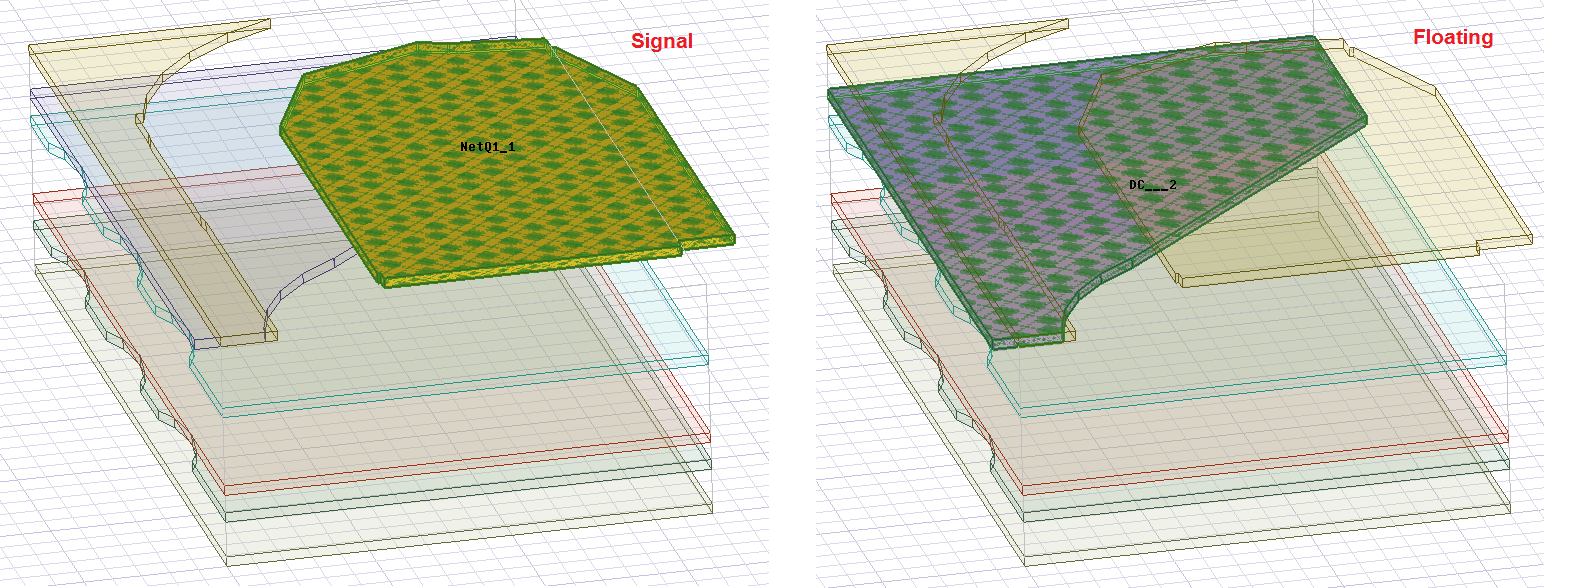
\includegraphics[width=\linewidth]{pictures/examples/Q1d_verified2.png}
  \caption{Q1-Gate set as Signal and Q1-Drain set as Ground}
  \label{fig:PCB_verified3}
\end{figure}

\item Next, similar to Section 6.2.2. Step 9, 'Validation Check' is done prior to analysis to check for any error with the design that might prevent the extraction process

\item If, 'Validation Check' returned no error, similar to Section 6.2.2. Step 10, after adding 'Solution Setup', the final step, which is 'Analysis' is carried out to extract the parasitic components.

\begin{figure} [H]
  \centering
  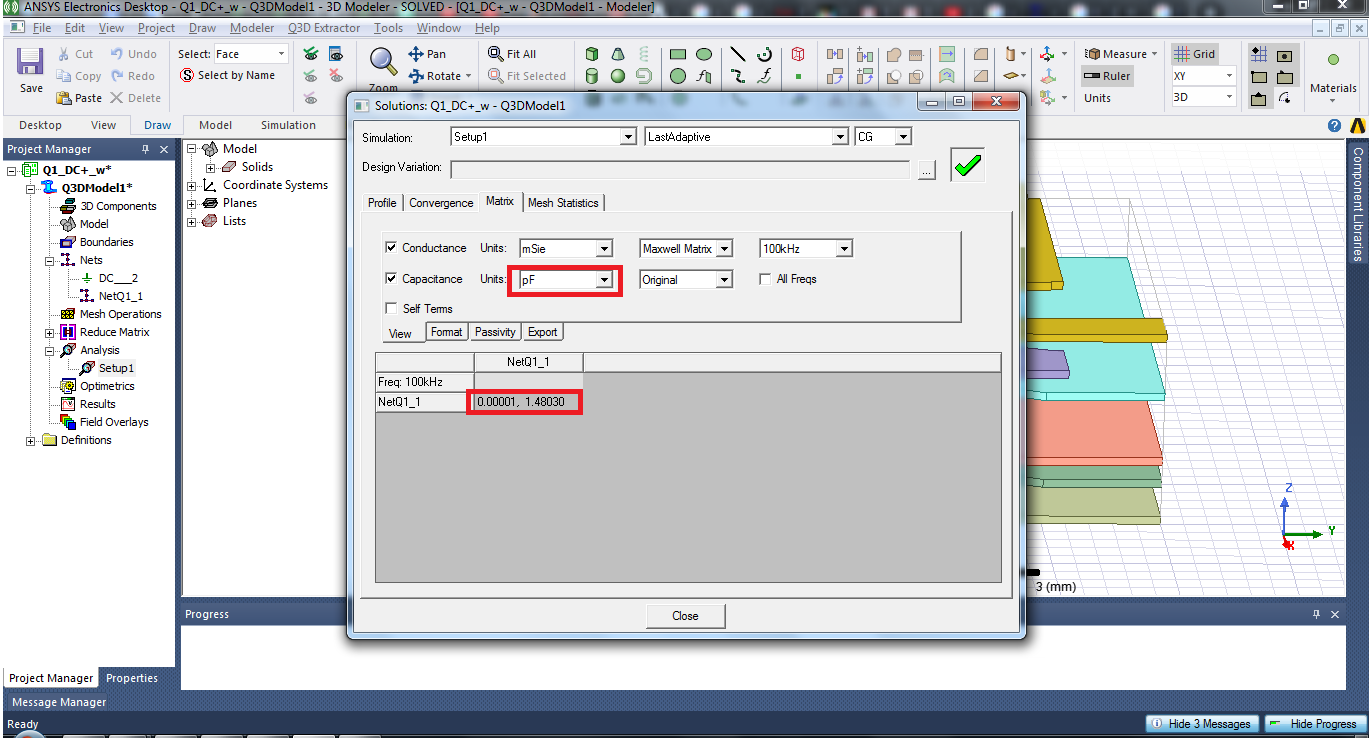
\includegraphics[width=\linewidth]{pictures/examples/results2.png}
  \caption{Solution showing the parasitic components}
  \label{fig:results2}
\end{figure}

\item In the end, the extracted parasitic component is collected and added to the SPICE model. Parasitic capacitance from other areas where the nets overlap as shown in Section 6.5 (Q1 gate and source, Q1 drain and source, Q3 gate and drain, Q3 gate and source, Q3 drain and source) are extracted using similar method and when all are solved, analysis is done on the SPICE model to compare between the ideal model (without the parasitic components) and the extracted model (with the parasitic components).

\begin{figure} [H]
  \centering
  \includegraphics[width=\linewidth]{pictures/examples/spice6.png}
  \caption{Parasitic capacitance added to the spice model}
  \label{fig:results2}
\end{figure}

\end{enumerate}

Parasitic capacitance extracted between other nets are given in Section 6.5.